
%: ----------------------- introduction file header -----------------------
\begin{savequote}[50mm]
Historical methodology, as I see it, is a product of common sense applied to circumstances. 
\qauthor{Samuel E. Morison}
\end{savequote}


\chapter{The AdaptUI System Architecture}
\label{cha:architecture}

\ifpdf
    \graphicspath{{4_system_architecture/figures/PNG/}{4_system_architecture/figures/PDF/}{4_system_architecture/figures/}}
\else
    \graphicspath{{4_system_architecture/figures/EPS/}{4_system_architecture/figures/}}
\fi

During this dissertation several problems of adaptive systems have been remarked.
Special attention has been paid to their lack of dynamism, the problems of 
modelling (\textit{what} and \textit{how} to model, the \textit{depth} of the 
model and the \textit{required knowledge} in the domain) and the external 
services and platforms dependency to perform computational complex operations. 
Addressing these issues, this dissertation aims a fully operational mobile 
platform. This chapter describes the three-layered architecture designed for 
the AdaptUI platform. The architecture layers and their modules are depicted in 
Figure~\ref{fig:architecture}.

Each layer of the AdaptUI platform is composed of several modules; each module
aiming to solve a concrete requisite. First, there is the Modelling Layer which
collects information of the user's (non physiological) capabilities and context
and device characteristics to finally build a semantic representation of this
knowledge. Two main modules form the Modelling Layer: the Capabilities Collector
and the Semantic Modeller. On the one hand, the Capabilities Collector's main
goal is to obtain information about each entity. On the other hand, the Semantic
Modeller leads the semantic representation and storage of the information
collected by the Capabilities Collector.

Next, there is the Adaptation Layer, which manages the adaptation process of the
user interface components through the Adaptation Engine. Together with the
Adaptation Engine there is the Adaptation Polisher module. This module aims to
refine the adapted user interface by analysing several usability metrics of the
user interaction.

Finally, there is the Application Layer. This layer provides several tools for
developers to be able to use AdaptUI. Through the provided \ac{api} developers 
are allowed not only to make their applications adaptive, but also to add, edit 
and delete knowledge and rules.

\begin{figure}[H]
\centering
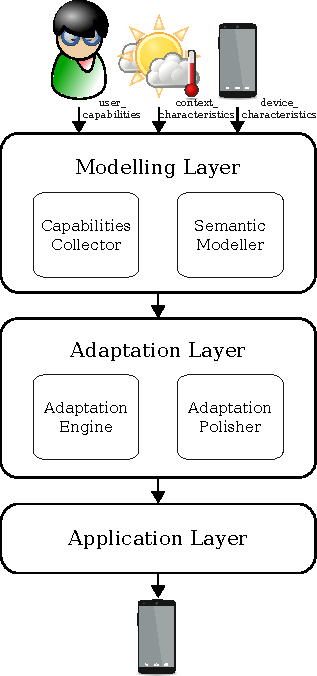
\includegraphics[width=0.30\textwidth]{architecture.pdf}
\caption{AdaptUI's three-layered global architecture.}
\label{fig:architecture}
\end{figure}

In the next sections of this chapter each layer and module is more concretely
explained. First, in Section~\ref{sec:modelling_layer} the Modelling Layer and
its two modules are introduced. The Capabilities Collector is described in
Section~\ref{sec:capabilities_collector}, while the Semantic Modeller is 
detailed in Section~\ref{sec:semantic_modeller}. The Adaptation Layer is 
presented in Section~\ref{sec:adaptation_layer}. This section also details the 
Adaptation Polisher (see Section~\ref{sec:adaptation_polisher}). Next,
Section~\ref{sec:application_layer} presents the characteristics of the 
Application Layer.

In addition, in Section~\ref{sec:architecture_flow}, the relationships among 
the mentioned layers and modules and the flow of the information and knowledge 
within the AdaptUI platform is depicted. Finally, a detailed example is
described in Section~\ref{sec:complete_example} following the information flow
mentioned in Section~\ref{sec:architecture_flow}, highlighting the concrete
tasks performed by each layer and module.


% At the end of this section (in Section~\ref{sec:architecture_flow}), after
% describing each layer and module, the information flow within the whole AdaptUI
% platform is described. 

\section{The Modelling Layer}
\label{sec:modelling_layer}

The first layer to be described of the AdaptUI architecture is the Modelling
Layer. This layer aims to generate the different profiles (semantic models) for
the three main entities: the user, the current context and the device. In order
to do this, the Modelling Layer combines the results of two different modules: 
the Capabilities Collector and the Semantic Modeller. The Capabilities Collector
collects information about the three main entities. This module deals with the
current capabilities of the user, the environment current situation, and with
several characteristics of the device, storing the collected information for
further usage. On the other hand, the Semantic Modeller represents the knowledge
gathered and stored by the Capabilities Collector in a semantic model specified
at the AdaptUIOnt ontology (which is fully described in 
Chapter~\ref{cha:ontology_model}). 

The two modules which form the Modelling Layer are described in the following
sections. First, the Capabilities Collector is introduced in
Section~\ref{sec:capabilities_collector}. Next, the Semantic Modeller is
presented in Section~\ref{sec:semantic_modeller}.


\subsection{The Capabilities Collector}
\label{sec:capabilities_collector}

As cited in the literature, \citet{fischer_user_2001} defended that the user
evolves through time. More concretely, time and experience are two of the 
reasons for the cited evolution of user's characteristics. In AdaptUI users 
evolve, but under different assumptions. Fischer considered long terms 
parameters as the keys for the evolution of the user. On the contrary, AdaptUI 
takes into account temporary and concrete context conditions, limited to a 
specific momentum. Consequently, the user model is built contemplating a dynamic 
user whose capabilities change due to context conditions.

Considering this dynamic user perspective, based in several aspects related to
context terms, we discussed how this could be applicable to mobile devices. 
Mobile devices have several characteristics that make them susceptible to change 
(i.e., battery consumption, location awareness, preferences of the screen or 
sound). Thus, in AdaptUI mobile devices are also considered as a dynamic entity.

Finally, regarding the surrounding environment, we consider that it also has the 
propensity to change (i.e., temperature, light or noise). Therefore, within the 
Modelling Layer a concrete module to collect these characteristics has been 
designed: the Capabilities Collector.

The Capabilities Collector is a software module that allows the system gathering 
non physiological capabilities of the user, collect different variables of the 
current environment situation, and identify several device characteristics in 
order to be aware of the whole domain limitations.

Figure~\ref{fig:capabilities_collector_flow} illustrates how the Capabilities 
Collector uses several activities to collect the information about the three 
entities. Next this information is transferred to the Semantic Modeller.

\begin{figure}
\centering
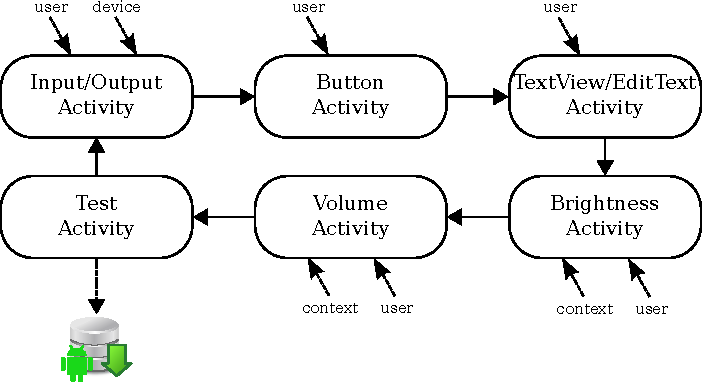
\includegraphics[width=0.65\textwidth]{capabilities_collector_flow.pdf}
\caption{The Capabilities Collector activities and their relationships with the
three main entities in AdaptUI.}
\label{fig:capabilities_collector_flow}
\end{figure}


\subsubsection{Android Activity}
\label{sec:activities}

In Android, activities are application components that provide a screen with
which the user can interact. Each activity is given a window in which to draw
its user interface. Android applications usually consist of multiple activities 
that bound to each other. 

Android applications have to declare a Main activity. This activity is always
presented to the user when launching the application for the first time. Besides,
activities can start other activities storing their current status (if needed).
An activity lifecycle is illustrated in Figure~\ref{fig:activity_lifecycle}.

\begin{figure}
\centering
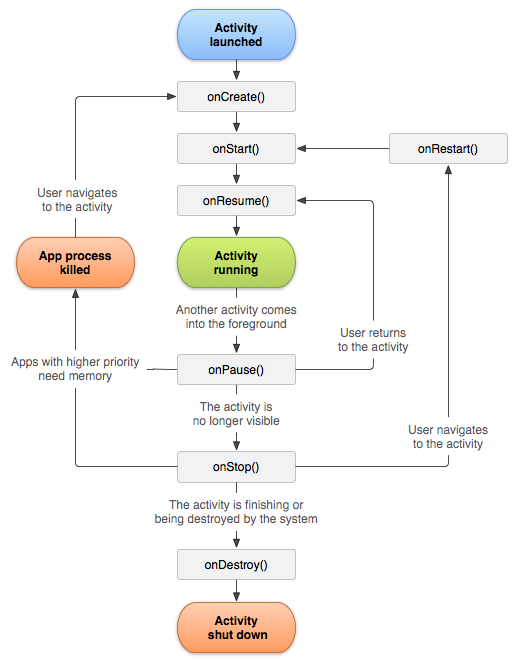
\includegraphics[width=0.65\textwidth]{activity_lifecycle.png}
\caption{The activity lifecycle~\citep{activities}.}
\label{fig:activity_lifecycle}
\end{figure}

Creating activities is easy. Extending the Activity class~\citep{activities},
a main callback method is needed to be implemented: the onCreate() method. The
system always calls this method when creating an activity. In it, the essential
components of the activity should be initialized. Besides, and before any
initialization, the setContentView() method has to be called. This method defines
the layout for the activity's user interface, which is defined as an \ac{xml}
file in the \textit{layout} folder of the Android project.

Listing~\ref{lst:android_activity} shows an example of an activity initialization.
The layout of the activity is shown in Listing~\ref{lst:activity_layout}. Next,
Figure~\ref{fig:android_activity} illustrates the result of such activity.

\inputminted[linenos=true, fontsize=\footnotesize, frame=lines]{java}{4_system_architecture/android_activity.java}
\captionof{listing}{Example of an activity initialized with a button.\label{lst:android_activity}}

\inputminted[linenos=true, fontsize=\footnotesize, frame=lines]{xml}{4_system_architecture/activity_layout.xml}
\captionof{listing}{An activity layout declaring a button.\label{lst:activity_layout}}

\begin{figure}
\centering
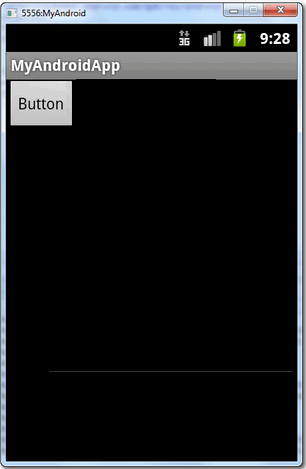
\includegraphics[width=0.35\textwidth]{android_activity.png}
\caption{The resulting activity from the combination of Listing~\ref{lst:android_activity} and
Listing~\ref{lst:activity_layout}.}
\label{fig:android_activity}
\end{figure}

It is also important to remember defining the activity in the \textit{AndroidManifest.xml}
file. This file gathers the main specification of the declared activities, filters,
services and allowed permissions, along with the identification of the application.
Listing~\ref{lst:android_manifest} shows an example of a typical manifest file.

\inputminted[linenos=true, fontsize=\footnotesize, frame=lines]{xml}{4_system_architecture/android_manifest.xml}
\captionof{listing}{Application manifest file.\label{lst:android_manifest}}

\subsubsection{Collecting the user's capabilities}
\label{sec:user_capabilities}

AdaptUI requires the user's capabilities (together with the current context
situation and the characteristics of the mobile device) as an input  for the
adaptation process. As explained in Section~\ref{sec:entities_model}, the user
model of the AdaptUIOnt model does not consider physiological knowledge about
the user. This is due to the lack of physiological and medical background that
users (and developers) of AdaptUI might have, which makes the capabilities
representation inaccurate and impractical. Instead of this, the user model
within the AdaptUIOnt ontology provides a layer of abstraction, focusing on the
user interaction needs. For example, a user who suffers from a hearing disability
in AdaptUI can explicitly configure a minimum sound level, so the system will
not reduce it in any future adaptation. Thus, we avoid modelling specific
physiological problems related to the user's hearing capability. To collect this
kind of information about the user, the Capabilities Collector shows several
screens (known as activities in Android) to the user in which different
interactions are required. Android activities are explained in Section~\ref{sec:activities}.

The first capability that the Capabilities Collector deals with is the input
method or type of interaction. In the AdaptUIOnt ontology this is represented
through the \textit{Interface} class. Through several basic instructions
(presented in text mode and as quick audio question) the user selects his/her
input and output preferences. For example, Figure~\ref{fig:input_activity} shows
the first activity of the Capabilities Collector module. The instructions shown
in this activity can be read by the user and by the application itself (for
example, by using the Android Text-To-Speech~\citep{tts} service). Every decision
the user makes is stored in the mobile phone as a profile for a future
\textit{semantization} by the Semantic Modeller.

\begin{figure}
\centering
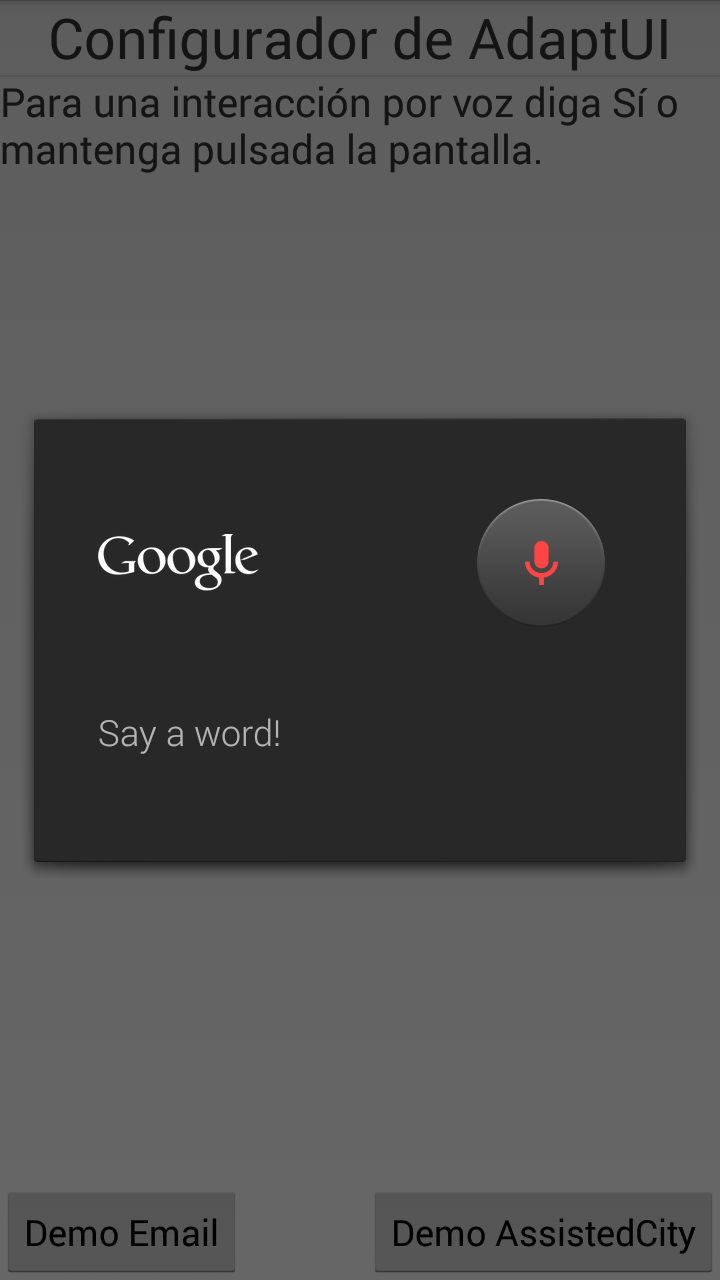
\includegraphics[width=0.35\textwidth]{input_activity.png}
\caption{Capabilities Collector's input activity.}
\label{fig:input_activity}
\end{figure}

Once the input interaction type has been determined the output is configured 
accordingly. Next activities show several Android view~\citep{android_view} 
components which are configurable by the user. Views represent the basic 
building block for user interface components in Android. A view occupies a 
particular area on the screen and is responsible for drawing and event 
handling~\citep{android_view}. In this case, a Button, a TextView and an 
EditText (which is a particular case of a TextView) are presented (see 
Figure~\ref{fig:views_activity}). The Capabilities Collector allows the user to 
modify their size, component colour, and also the text size and colour.

\begin{figure}
\centering
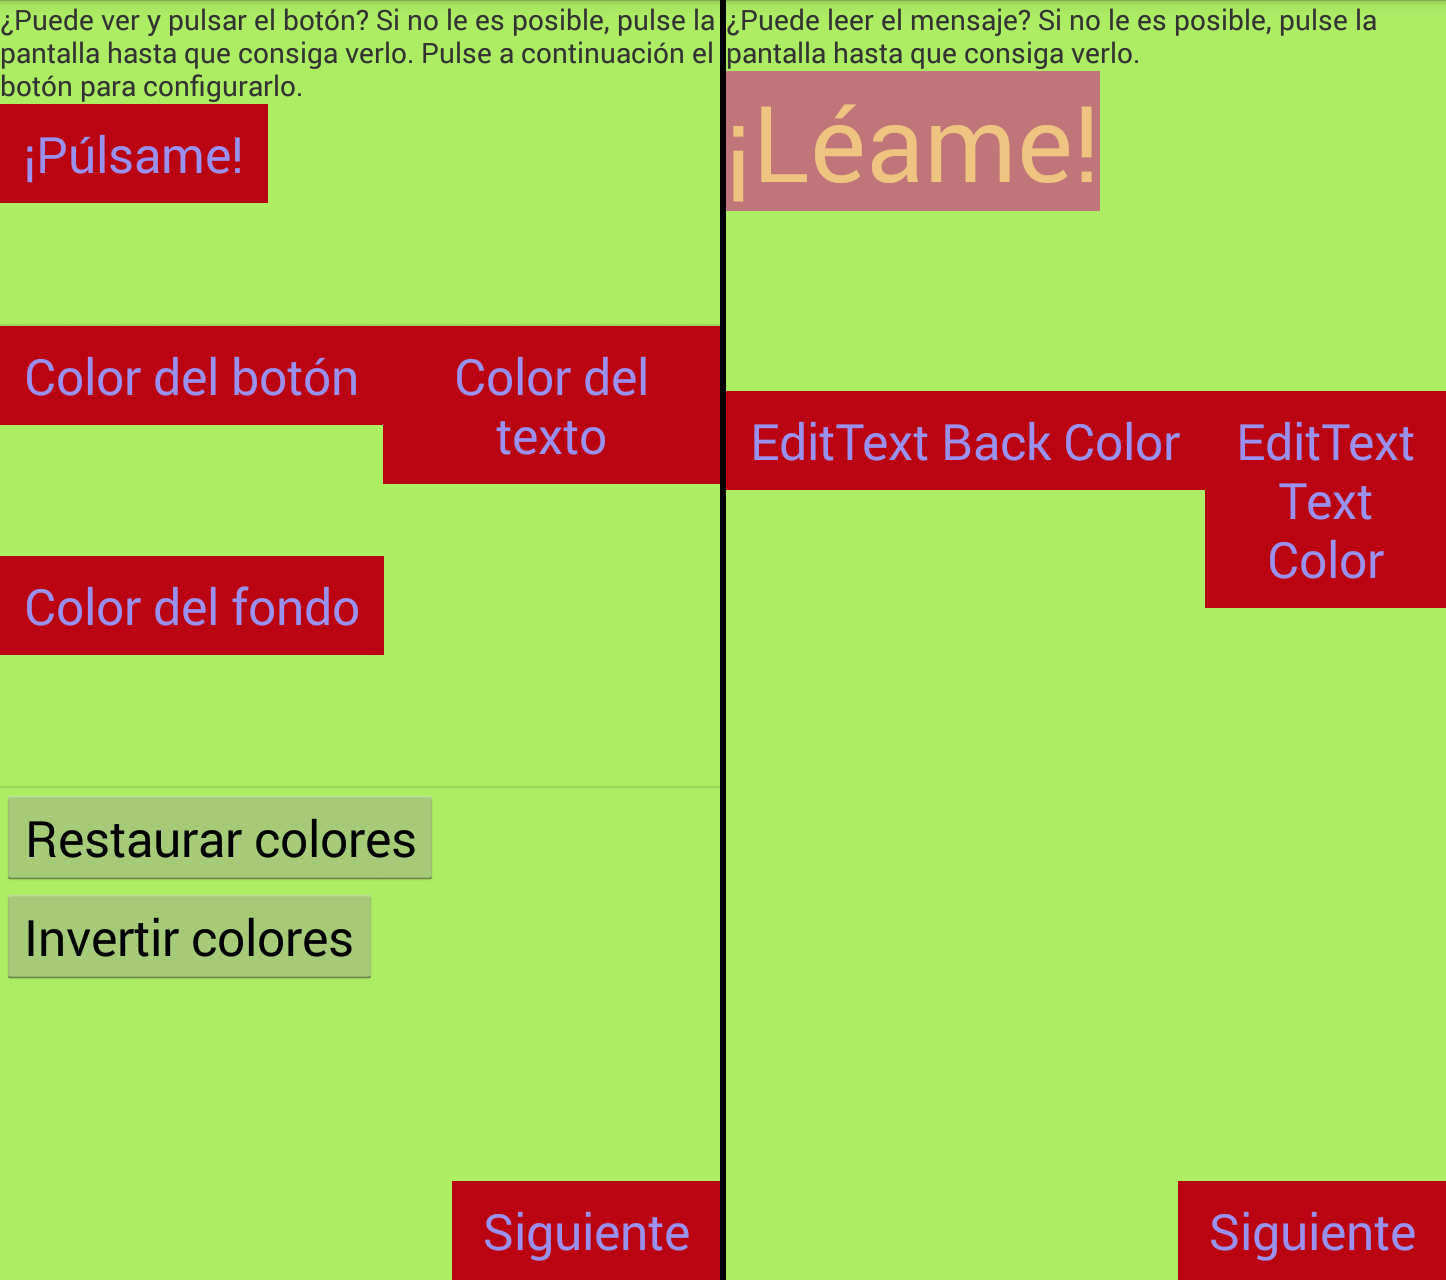
\includegraphics[width=0.65\textwidth]{views_activity.png}
\caption{Different Android view components
personalization: on the left, Button; on the right, TextView and EditText.}
\label{fig:views_activity}
\end{figure}

Finally, the display brightness and the system volume are also allowed to be
customized. The surrounding light and noise are monitored. Thus, AdaptUI is
aware of the context conditions and is able to adjust these parameters to 
the user's preferences.

 
\subsubsection{The context situation}
\label{sec:context_situation}
Current smartphones are equipped with several sensors that allow devices to
collect different environment parameters. Light sensors, microphones, proximity 
sensors for disabling the screen, even Bluetooth and infra-red transceivers are 
just several examples of the hardware available in such devices.

Taking advantage of the current situation, in which smartphones are able to sense
the environment, the Capabilities Collector collects knowledge of the user context.
Light conditions and noise are classified by the Capabilities Collector as follows:

\begin{itemize}
 \item Light conditions are measured in \ac{lx}, which is the \ac{si} unit of 
 luminance.
 
 \item The current noise is collected using the mobile available microphones. It
 is measured in \ac{db}, which is a logarithmic unit that expresses the ratio
 between two values of a physical quantity (often power or intensity).
\end{itemize}

Once all this features have been collected, the profile is temporarily stored in 
the device. This storage is carried out using the Android 
SharedPreferences~\citep{shared_preferences}. This class provides a general 
persistence framework for developers to save and retrieve key-value pairs of 
primitive data types. After this temporary storage in the device, the Semantic 
Modeller is the module which deals with the task of the semantic representation 
of the model. Listing~\ref{lst:shared_preferences} shows how developers deal 
with the SharedPreferences to store and retrieve data in Android. If complex
objects need to be stored, the process is different (see Listing~\ref{lst:shared_preferences_complex}).

\inputminted[linenos=true, fontsize=\footnotesize, frame=lines]{java}{4_system_architecture/shared_preferences.java}
\captionof{listing}{Using Android SharedPreferences. By default SharedPreferences allows 
to store and retrieve primitive data. Implementing Parcelable allows complex 
objects to be persistent.\label{lst:shared_preferences}}

\inputminted[linenos=true, fontsize=\footnotesize, frame=lines]{java}{4_system_architecture/shared_preferences_complex.java}
\captionof{listing}{Using Android SharedPreferences to store non primitive
objects.\label{lst:shared_preferences_complex}}

Figure~\ref{fig:context_activity} shows how the brightness and the volume of
the application is configured by an user which is aware of the light and noise
of the environment.

\begin{figure}
\centering
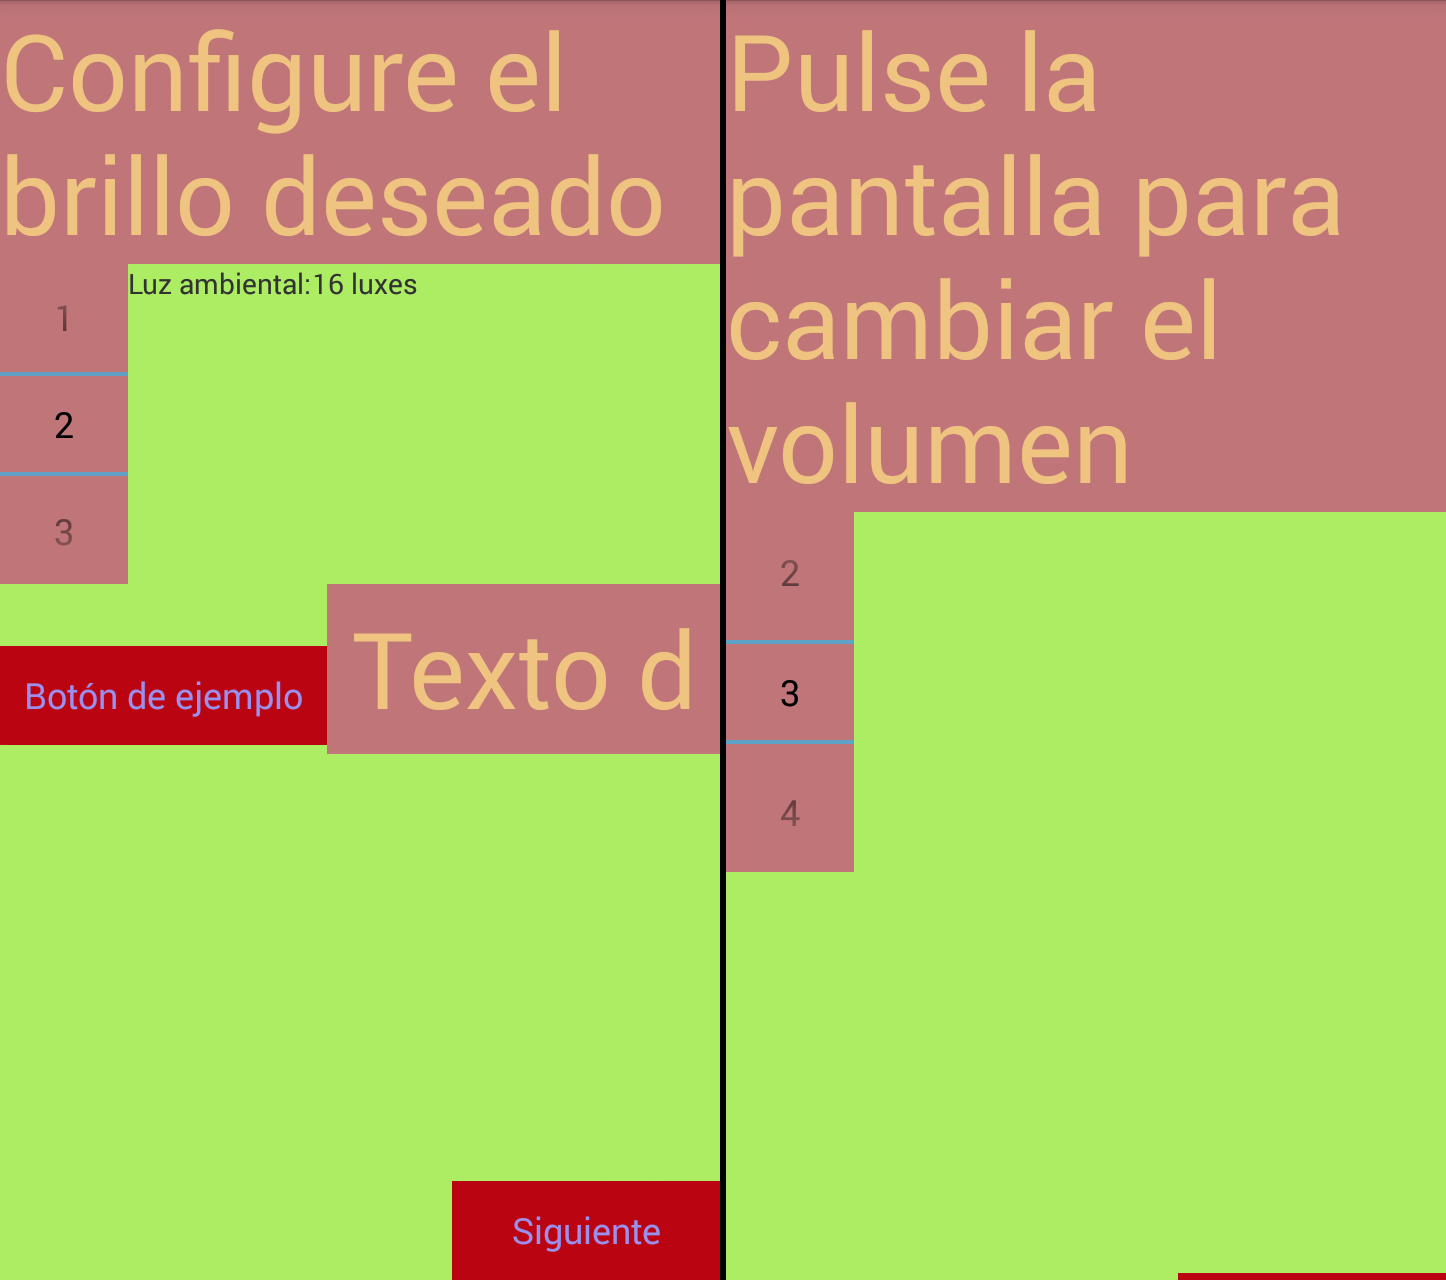
\includegraphics[width=0.65\textwidth]{context_activity.png}
\caption{Brightness (left) and Volume (right) adjustment sensing the surrounding
light and noise.}
\label{fig:context_activity}
\end{figure}


\subsubsection{The device characteristics}
\label{sec:device_characteristics}

Device characteristics are significant within the AdaptUI platform. These
characteristics limit the possible adaptations of the user interface. For example,
not all the smartphones have the same maximum brightness or sound levels, nor
they have the same connectivity capabilities. Thus, being aware of each device's
capabilities becomes essential in AdaptUI.

The device characteristics are collected by the Capabilities Collector by using
the \textit{Settings.System} class in Android. This class contains global
system-level device preferences. Listing~\ref{lst:device_settings_brightness} 
shows a piece of code which requests the maximum values for the brightness. To 
allow the user to change the brightness of the device's screen a NumberPicker 
element is shown. In its initialization, it is needed to specify the minimum and 
the maximum values of the range. Thus, the user is able to configure the brightness 
to $0$. For the maximum brightness value it is needed to state a default value 
of $1F$.

\inputminted[linenos=true, fontsize=\footnotesize, frame=lines]{java}{4_system_architecture/device_settings_brightness.java}
\captionof{listing}{Android NumberPicker initialization with a minimum value of 0 and a 
maximum value requested to the Settings.System class.\label{lst:device_settings_brightness}}


On the contrary, to get values related to audio, the \textit{AudioManager} class
is required. Listing~\ref{lst:device_settings_volume} shows a piece of code with
which the developer initializes a NumberPicker with the minimum and maximum
volume levels available in the current device.

\inputminted[linenos=true, fontsize=\footnotesize, frame=lines]{java}{4_system_architecture/device_settings_volume.java}
\captionof{listing}{Android NumberPicker initialization with a minimum value of 0 and a 
maximum value requested to the AudioManager class.\label{lst:device_settings_volume}}


Before asking the user about the way of interaction, the Capabilities Collector
performs an analysis about several device's capabilities. Several hardware
details are collected: processor maximum speed, processor availability, battery
current levels, maximum and current available memory, available input modes, 
and so forth. All the characteristics are shown in Table~\ref{tbl:device_characteristics}. 
These are stored during the process for the Semantic Modeller to store in the 
final model.

\begin{table}[H]
  \caption{Requested device characteristics.}
 \label{tbl:device_characteristics}
\footnotesize
\centering
 \begin{tabular}{l l}
  \hline 
  \textbf{Characteristic}& \textbf{Description}				\\
  \hline
  Brightness		& Describes the current device’s brightness.	\\
  Contrast		& Represents the current device’s contrast.	\\
  Volume		& Describes the current device’s volume.	\\
  Processor		& Models the number of the device’s cores.	\\
  OS version		& Indicates the current	\ac{os} version.	\\
  Acceleration		& Represents the current X, Y, Z acceleration.	\\
  Orientation		& Current orientation of the device.		\\
  Device memory		& Maximum device memory.			\\
  Available memory	& Current available device memory.		\\
  Battery		& Current device battery levels.		\\
  Screen resolution	& Maximum screen resolution.			\\
  Storage		& Maximum available storage.			\\
  Available storage	& Current available storage.			\\
  Processor		& Maximum processor of the device.		\\
  Available processor	& Current processor availability.		\\
  \hline
\end{tabular}
\end{table}


\subsection{The Semantic Modeller}
\label{sec:semantic_modeller}

Once the Capabilities Collector has finished its task, all the collected
knowledge is stored in the mobile. The Semantic Modeller's goal is to build a 
semantic representation of this knowledge through the AdaptUIOnt ontology and
store it in the mobile device. This task requires from a semantic reasoner. 
However, there are no available and remarkable reasoners written in Java and 
compatible with Android. Thus, an Android port of the 
Pellet~\citep{pellet} reasoning engine has been developed: \textit{Pellet4Android}.

During the following subsections both versions of the Pellet reasoning engine
are presented. First, in Section~\ref{sec:pellet}, the Java based Pellet reasoning
for desktop is introduced. Next, Section~\ref{sec:pellet4android} describes the
process followed to port Pellet to Android.

As the Semantic Modeller finishes storing the corresponding knowledge in the
AdaptUIOnt ontology, several rules are triggered. The main consequence of the
execution of these rules is shown through the \textit{Adaptation} class. This
class is filled with the adaptation values that will be requested by the
Adaptation Layer, which is the next layer of the AdaptUI architecture.


\subsubsection{Pellet}
\label{sec:pellet}

% \begin{description}
%   \item[\Defi{Reasoner by~\citet{owlapi_reasoners}}] \hfill \\
%   \begin{mdframed}[hidealllines=true,backgroundcolor=gray!20]
%   \textit{``A reasoner is a key component for working with \ac{owl} ontologies. 
%   In fact, virtually all querying of an \ac{owl} ontology (and its imports closure) 
%   should be done using a reasoner. This is because knowledge in an ontology 
%   might not be explicit and a reasoner is required to deduce implicit knowledge 
%   so that the correct query results are obtained''}~\citep{owlapi_reasoners}.
%   \end{mdframed}
% \end{description}

Developed by Clarkparsia, Pellet is a free and open source \ac{owl}-\ac{dl}
reasoner written in Java. As a \ac{dl} reasoner, it provides several standard 
inference services~\citep{pellet}:

\begin{itemize}
  \item \textit{\ac{owl}-\ac{dl} consistency checking}: Pellet assures that the 
  knowledge represented in the ontology does not contain contradictory facts. 
  \citet{carroll_owl_2004} define that \textit{an \ac{owl} consistency checker 
  takes a document as input, and returns one word being Consistent, Inconsistent, 
  or Unknown.} In \ac{dl} terminology  this is the operation to check the 
  consistency of an ABox with respect to a TBox (see the description of this 
  \ac{dl} terminology in Table~\ref{tbl:dl_terms}).
  
  \item \textit{Concept satisfiability}: Determines whether it is possible for 
  a class to have any instances. This avoids cases in which unsatisfiable classes 
  might define instances, which will cause the ontology to be inconsistent.
  
  \item \textit{Classification}: Pellet is able to create the complete class 
  hierarchy from the the computation of the subclasses relations between every 
  named class. This allows performing future queries (i.e., getting all the 
  direct subclasses of a class).
  
  \item \textit{Realization}: It is able to find the most specific classes that 
  an individual belongs to. Realization directly depends on classification, and 
  it cannot be done without it.
\end{itemize}


\begin{table}[H]
  \caption{Several \ac{dl} terminology.}
 \label{tbl:dl_terms}
\footnotesize
\centering
 \begin{tabular}{l l}
  \hline 
  \textbf{Component} 		& \textbf{Description}				\\
  \hline
  ABox (Assertional Box)	& Contains assertions about individuals	\\
				& (i.e., \ac{owl} facts such  as type, property	\\
				& -value, equality or inequality assertions).	\\
  TBox (Terminological Box)	& Contains axioms about classes, i.e., \ac{owl}	\\
				& axioms such as subclass, equivalent class 	\\
				& or disjointness axioms.			\\
  \acl{kb}			& A combination of ABox and TBox (i.e.,		\\
				& a complete ontology).				\\
  \hline
  
\end{tabular}
\end{table}

The reasoning capabilities of Pellet are accessible through different 
interfaces. For example, Pellet is directly integrated with the Protégé ontology 
editor~\citep{protege}. Thus, reasoning capabilities are allowed through the 
user interface of this editor. For developers, there are several tools provided 
as \acsp{api} which allow the utilisation of Pellet. The most significant ones 
are Apache Jena~\citep{jena} and Manchester \ac{owl}-\ac{api}~\citep{owlapi}:

\begin{itemize}
  \item Jena: Apache Jena (or Jena) is a free and open source framework written
  in Java which allows building semantic web and Linked Data applications. The
  framework is composed of different \acp{api} interacting together to process 
  \ac{rdf} data.
  
  \item \ac{owl}-\ac{api}: Available under \ac{lgpl} or Apache Licenses, the 
  \ac{owl}-\ac{api} is an open source high level \ac{api} maintained by the 
  University of Manchester for working with \ac{owl} ontologies. Closely aligned 
  with the \ac{owl} 2 structural specification, the \ac{owl}-\ac{api} supports 
  parsing and rendering in the syntaxes defined in the \ac{w3c} specification 
  (i.e., Functional Syntax, \ac{rdf}/\ac{xml}, \ac{owl}/\ac{xml} and the 
  Manchester \ac{owl} Syntax), the manipulation of ontological structures, and 
  the use of reasoning engines (i.e., Chainsaw, FaCT++, JFact, HermiT, Pellet 
  and RacerPro).  
\end{itemize}

% The core of the system is the tableaux reasoner. This reasoner checks the
% consistency of a knowledge base and allows Pellet to support \ac{swrl}~\citep{swrl}
% rules language.


\subsubsection{Reasoning with Pellet in Android: Pellet4Android}
\label{sec:pellet4android}

The AdaptUI platform was conceived to support reasoning and semantic knowledge
representation due to the benefits that ontologies bring. Nevertheless, after
analysing the possibilities and solutions provided by the community (i.e., mobile
reasoning platforms) we found that, although nowadays mobile capabilities allow
heavier processing, there are no remarkable efforts in the area.

\citet{yus_android_2013} noticed this issue and made great efforts porting
several Java based reasoners to Android. Although the authors do not provide the
developed ports to the community, they do provide the instructions they followed
to make these reasoners available for Android devices. Thus, following these
directions a port of Pellet has been developed for AdaptUI: \textit{Pellet4Android}.

As Pellet, \textit{Pellet4Android} also supports full \ac{owl} 2 and \ac{dl} 
rules. To make Pellet run in Android the following steps were needed:

\begin{itemize}
  \item Pellet uses Jena, which is a free and open source framework written in
  Java which allows building semantic web and Linked Data applications. However,
  Jena is not directly importable to Android. Thus, it is necessary to replace it
  with Androjena~\citep{androjena}. Androjena is a porting of Hewlett-Packard's
  Jena semantic web framework to Android. 
  
  \item Pellet also imports the \ac{jaxb} library~\citep{jaxb} for \ac{xml} 
  parsing. \ac{jaxb} is able to translate \ac{xml} Schemas building a set of 
  classes that correspond to that schema. It originally comes with the Java 1.6 
  release, but its easily importable to previous Java version integrating the 
  \ac{jaxb} jar files. The problem is that \ac{jaxb} uses classes that are not 
  compatible with Android. Thus, this package has been removed. 
  
  \item As the official Oracle documentation states, the \textit{javax.xml.bind}
  package \textit{``provides a runtime binding framework for client applications
  including unmarshalling, marshalling, and validation capabilities''}~\citep{javax_xml_bind}.
  Nevertheless, this package is also incompatible with Android, and we should
  remove it from the package list and the build path.
  
  \item Also related with the way Java manages \ac{xml} files, the 
  \textit{org.apache.xerces}~\citep{xerces} package is used for the creation and 
  maintenance of \ac{xml} parsers and related software components. Several 
  classes under this package are not importable by Android, so the package has 
  to be removed.
  
  \item Finally, under the \textit{com.clarkparsia.pellet} package there are several
  classes that are not directly importable by Android. Thus, without removing them,
  we have to search the specific troublesome lines of code (usually related with
  concrete data types and exceptions) and comment them. 
\end{itemize}

Figure~\ref{fig:pellet4android} shows the package structure of the
\textit{Pellet4Android} port and the imported libraries in the Android project.
% 
% \InsertFig{pellet4android}{fig:pellet4android}{Package structure (left) and 
% needed libraries (right) for Pellet4Android}{}{0.85}{}

\begin{figure}[H]
\centering
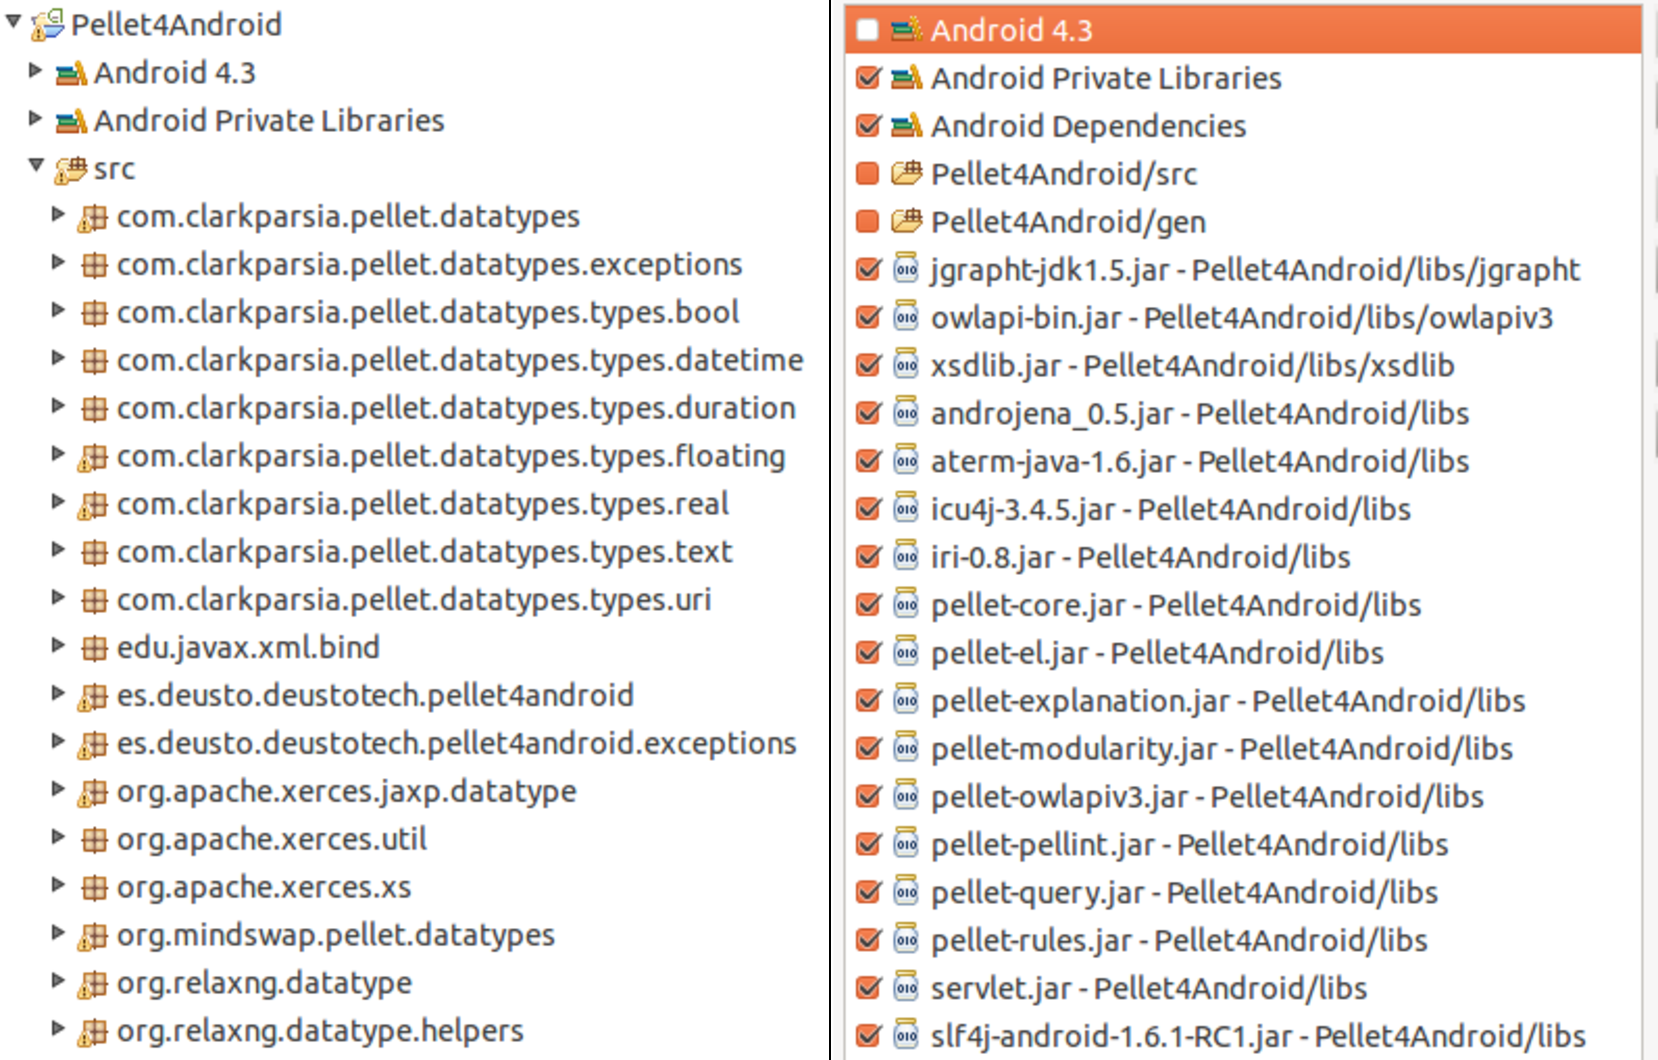
\includegraphics[width=0.85\textwidth]{pellet4android.pdf}
\caption{Package structure (left) and needed libraries (right) for Pellet4Android.}
\label{fig:pellet4android}
\end{figure}


As~\citet{yus_android_2013} remarked, it is important to provide a larger heap
size. To do this, the \textit{android:largeHeap} tag of the AndroidManifest.xml 
file of the project has to be changed to \textit{true}.

A first evaluation of the port was carried out by~\citet{yus_android_2013}.
Nevertheless,~\citet{bobed_android_2014} performed a second evaluation of the
Pellet version for Android obtaining promising results in terms of efficiency
and time responsiveness. Although in this dissertation a similar approach to port 
Pellet has been followed, it is impossible to be a 100\% sure if the results are 
the same (as the version by~\citet{yus_android_2013} was not available for testing). 
Thus, in Chapter\ref{cha:evaluation} an evaluation of \textit{Pellet4Android} is 
included.

As Pellet is available for open source applications under the terms of the AGPL
version 3 license, the provided \textit{Pellet4Android} is also available in
Github~\citep{pellet4android} under the same license regulations.


\section{The Adaptation Layer}
\label{sec:adaptation_layer}

The second layer of the AdaptUI architecture is the Adaptation Layer. After the
processes performed by the Modelling Layer, the Adaptation Layer aims to lead the
dynamic adaptation of the elements presented in the user interface. It is formed
by two different modules: The Adaptation Engine, which purpose is to adapt the
currently interface shown by the device, and the Adaptation Polisher, which aims
the refinement of the user interface basing its task in several usability metrics.


\subsection{The Adaptation Engine}
\label{sec:adaptation_engine}

After the storage of the domain knowledge in the AdaptUIOnt ontology by the
Semantic Modeller, several rules are triggered. These rules are grouped in three
different subsets: the pre-adaptation rules, the adaptation rules and the post-adaptation
rules. More concretely, the adaptation rules subset is the one which modifies
the knowledge represented by the \textit{Adaptation} class in the AdaptUIOnt
ontology.

Once these rules have been executed the Adaptation Engine requests these results
to the \textit{Adaptation} class. Then, it launches several methods to dynamically
change the aspect of the current user interface. These methods basically redraw
and refresh the different components shown in the current activity, sharing
their new characteristics to the rest of activities. 

Listing~\ref{lst:redraw} shows an example of how several views are redrawn.
First, the elements that are part of the activity (i.e., buttons and textviews)
are initialized (similarly to other applications). Next, several methods regarding
the adaptation are called. The \textit{redrawViews()} method takes into account
the user's configured profile through the Capabilities Collector and adapts the
components of the activity accordingly. Every activity overwrites this method
(and others), as they extend from a parent abstract class called
\textit{AbstractActivity}. This class mainly manages the services initialization
(e.g., TextToSpeech) and the ontology. Listing~\ref{lst:abstract_activity} shows
part of the AdaptUI source code where the ontology is initialized.


\inputminted[linenos=true, fontsize=\footnotesize, frame=lines]{java}{4_system_architecture/redraw.java}
\captionof{listing}{Example of the creation and adaptation of an activity. In this case 
the example is centred in the adaptation of a button.\label{lst:redraw}}

\inputminted[linenos=true, fontsize=\footnotesize, frame=lines]{java}{4_system_architecture/abstract_activity.java}
\captionof{listing}{The AbstractActivity class ontology related methods.\label{lst:abstract_activity}}

Listing~\ref{lst:store_in_ontology} shows a piece of code where the developer
uses the \ac{owl}-\ac{api} to store the user profile in the AdaptUIOnt model. 
The methods called in this example are part of the Turambar framework~\citep{david_ausin_probabilistic_2014}. 
This framework provides a high-level \ac{api} for managing the \ac{owl}-\ac{api}.

\inputminted[linenos=true, fontsize=\footnotesize, frame=lines]{java}{4_system_architecture/store_in_ontology.java}
\captionof{listing}{Inserting values in the corresponding classes of the AdaptUIOnt 
ontology.\label{lst:store_in_ontology_activity}}


Finally, Figure~\ref{fig:adaptation_differences} shows two activities with the
same user interface. The difference is that the activity on the left is showing
the default user interface defined in the activity's layout. On the contrary,
the activity on the right shows adapted components in its interface.

\begin{figure}[H]
\centering
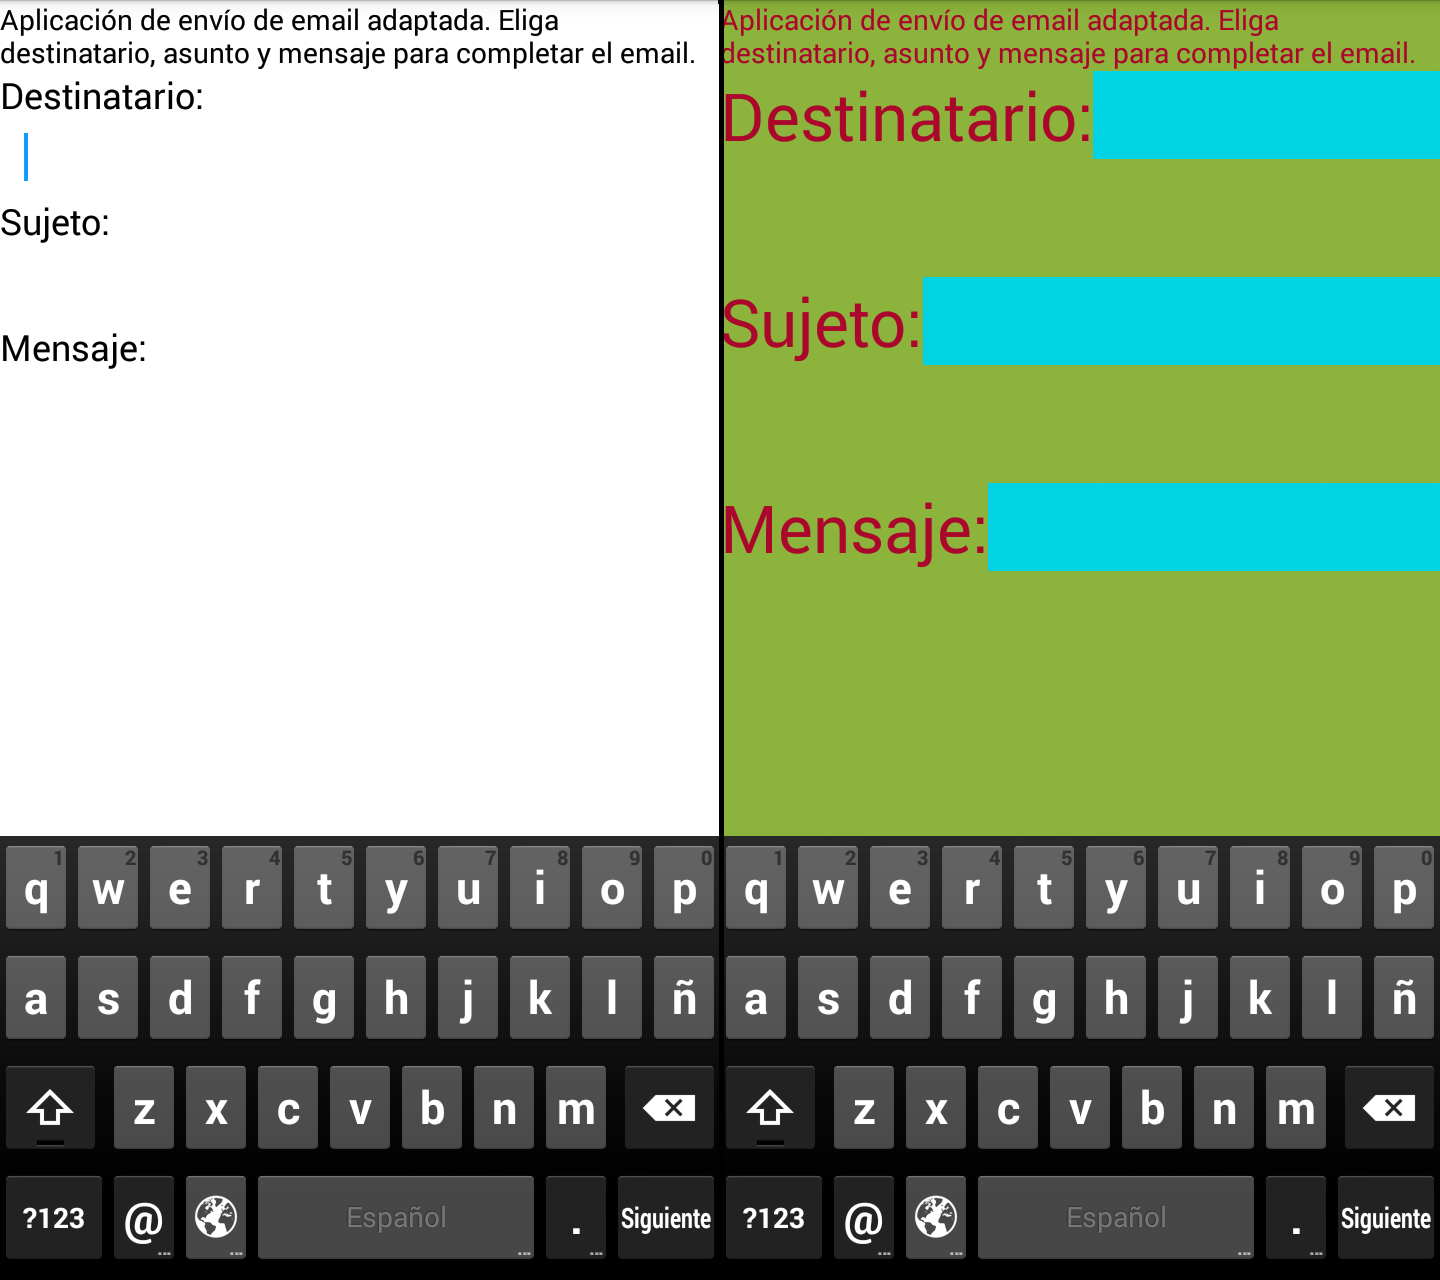
\includegraphics[width=0.65\textwidth]{adaptation_differences.png}
\caption{User interface adaptation performed by the Adaptation Engine. On the
left, a default activity with no adaptation. On the right, the same activity
after the adaptation process. As is shown, the colours sets and sizes of each
component of the adapted user interface are different from the non adapted one.}
\label{fig:adaptation_differences}
\end{figure}


\subsection{The Adaptation Polisher}
\label{sec:adaptation_polisher}

Although the adaptations for the user follow the instructions detailed by him/her,
there is still the possibility that the Adaptation Engine's results lead to a
unsuccessful interaction/adaptation. One of the main reasons for this is that
the classification of the model, considering the context aspects, is just an
approximation of the reality. For example, considering that between 1,000 \ac{lx} and
25,000 \ac{lx} the reasoner determines that the ontology value for the luminance
is \textit{daylight}, the difference might be significant in real scenarios
(see Table~\ref{tbl:luminance}). In other words, the user might easily interact
with a 1,000 \ac{lx} context light but tediously in a 24,999 \ac{lx} light environment. In
order to tackle this problem, there are two possible solutions: to consider
an extensive set of classification rules including more possible situations (e.g.,
dividing the luminance table into more categories), or to design a specific
module which evaluates the user interaction results: the Adaptation Polisher.

The first case is difficult to implement. Nevertheless, AdaptUI provides an \ac{api}
which aims to help in this issue allowing developers to create and modify the
ontology knowledge. This means that it is possible to try to model every tiny
context variation to capture different context characteristics and adapt the user
interface accordingly. However, this is not practical, and AdaptUI covers the
second case with the Adaptation Polisher. Therefore developers do not have to
model these small variations in the environment.

The Adaptation Polisher is a software module, part of the Adaptation Layer, which
monitors the effectiveness and responsiveness of the adapted interfaces. Collecting
different usability and productivity metrics of the interaction carried out by the
user, this module is able to make small but specific adaptations to improve
the ongoing interaction. This module has been designed considering the relative
user efficiency productivity metrics. These metrics compare the efficiency of the
user compared to an expert. But it has no sense to compare the user with others
in AdaptUI. The system cannot generalize and apply adaptations based on other
users' preferences. To solve this, in AdaptUI we propose to maintain a base
adaptation, which thanks to the Adaptation Polisher and its interaction results
will be improved. Consequently, an interaction model is built for each adaptation.
Therefore, we can determine the efficiency of the user when he/she is manipulating
an adaptation made by the system by comparing the last adaptation to the previous
one.

% AdaptUI keeps an interaction model of the user (as an expert) stored in the
% ontology. Once an adaptation is made, the Adaptation Polisher monitors the user
% interaction and then checks the stored model with the new generated one. Next,
% the post-adaptation rules are triggered.


\subsubsection{The usability metrics}
\label{sec:usability_metrics}
For this module, several usability metrics have been studied and implemented.
These metrics are classified into two different groups: effectiveness metrics
and productivity metrics.

Table~\ref{tbl:effectiveness_metrics} and Table~\ref{tbl:productivity_metrics}
detail the usability metrics implemented in AdaptUI. The following information
is given for each metric in the cited tables:

\begin{enumerate}[label=\alph*)]
  \item Purpose of the metric: Expresses the main goal of the current metric.
  \item Measurement, formula and data element computations: Provide the formulas
  to compute the current metric and the meaning of the used data elements.
  \item Interpretation of the measured value: Details the range and preferred values.
  \item Metric scale type: Provides the type of scale used by the current metrics.
  The possible scale types are: Nominal, Ordinal, Interval, Ratio and Absolute
  scale.
  \item Measure type: Provides the type of the measure. The possible measure
  types are: Size, Time and Count.
\end{enumerate}

In the original \ac{iso}document~\citep{ISOIEC9126} there are 4 extra columns that
have not been included in Table~\ref{tbl:effectiveness_metrics} and
Table~\ref{tbl:productivity_metrics}. This is because the values for each metric
under these columns are the same:

\begin{enumerate}[label=\alph*)]
  \item Method of application: Provides an outline of the application. 
  
  \item Input to measurement: Details the source of data used in the measurement.
  In this case there are two inputs that each metric shares: Operation (test) 
  report and User monitoring record.
  
  \item Reference: Identifies software life cycle processes where the metric is
  applicable. There are three processes that each metric shares: 6.5 Validation,
  5.3 Qualification testing and 5.4 Operation.
  
  \item Target audience: Identifies the user(s) of the measurement results. Again,
  the metrics share User and Human interface designer as their audiences.
\end{enumerate}


\myparagraph{Effectiveness metrics}
\label{sec:effectiveness_metrics}
Effectiveness metrics, as detailed in the \ac{iso}/\ac{iec} 9126-4~\citep{ISOIEC9126},
evaluate whether the current task achieves a specific goal considering the accuracy
and completeness of the corresponding task. These metrics are shown in
Table~\ref{tbl:effectiveness_metrics}.


% \begin{landscape}
\begin{table}
  \caption{The effectiveness metrics used in the Adaptation Polisher, as it appears in~\citep{ISOIEC9126}.}
 \label{tbl:effectiveness_metrics}
\footnotesize
\centering
 \begin{tabular}{l l l l l l}
  \hline 
\textbf{Metric}	& \textbf{Purpose of }	& \textbf{Measurement,}		& \textbf{Interpretation }	& \textbf{Metric}	& \textbf{Measure} 	\\
\textbf{name}   & \textbf{the metrics}	& \textbf{formula and data}	& \textbf{of measured }		& \textbf{scale}   	& \textbf{type}		\\
		& 			& \textbf{element compu-}	& \textbf{value}		& \textbf{type}					\\
		& 			& \textbf{tations}												\\
\hline
Task  		& To measure the 	& $M1=|1-\Sigma A_{i}|$		&  $0\leq M1 \leq 1$		& \textemdash 		& $A=$ proportion 	\\
effectiveness	& proportion of the  	& 				&				& 			& 			\\
		& goals of the task	& $A_{i}=$ proportional  	& The closer to			& 			& 			\\
		& achieved 		& value of each 		& 1.0 the better.		& 			& 			\\
		& correctly.		& missing or incorrect 		& 				& 			& 			\\
		& 			& component in the 	\\
		& 			& task output		\\
\hline	  
Task  		& To measure the 	& $X=A/B$			& $0\leq X \leq 1$    		& Ratio 		& $A=$ Count 		\\
completion 	& proportion of  	& 				& 				& 			& $B=$ Count		\\
		& the task that 	& $A=$ number of 		& The closer to			& 			& $X=$ Count/Count	\\
		& is completed.		& tasks completed		& 1.0 the better.		& 			& 			\\  
		& 			& $B=$ total number of		& 				& 			& 			\\
		& 			& tasks attempted	\\
\hline
Error  		& To measure the 	& $X=A/T$			& $0\leq X$  	  		& Absolute 		& $A=$ Count 		\\
frequency 	& frequency of 		& 				& 				& 			&~			\\
		& errors.		& $A=$ number of 		& The closer to			& 			&~			\\
		& 			& errors made by the 		& 0 the better.			& 			&~			\\  
		&			& user			\\
		& 			& $T=$ time or number 		& 				& 			& 			\\
		& 			& of tasks 		\\
\hline

\end{tabular}
\end{table}

% \end{landscape}


\myparagraph{Productivity metrics}
\label{sec:productivity_metrics}
Productivity metrics evaluate the resources consumed by the users in relation
to the effectiveness achieved in the current task~\citep{ISOIEC9126}. These 
metrics are shown in Table~\ref{tbl:productivity_metrics}.


% \begin{landscape}
\begin{table}
  \caption{The productivity metrics used in the Adaptation Polisher, as it appears in~\citep{ISOIEC9126}.}
 \label{tbl:productivity_metrics}
\footnotesize
\centering
  \begin{tabular}{l l l l l l}
  \hline 
\textbf{Metric}	& \textbf{Purpose of }	& \textbf{Measurement,}		& \textbf{Interpretation }	& \textbf{Metric}	& \textbf{Measure} 	\\
\textbf{name}   & \textbf{the metrics}	& \textbf{formula and data}	& \textbf{of measured }		& \textbf{scale}   	& \textbf{type}		\\
		& 			& \textbf{element compu-}	& \textbf{value}		& \textbf{type}					\\
		& 			& \textbf{tations}												\\
\hline
Task  		& To measure the 	& $X=Ta$			& $0\leq X$			& Interval 		& $T=$ Time	 	\\
time		& required time to	& 				&				& 			& 			\\
		& complete the task.	& $Ta=$ Task time		& The closer to			& 			& 			\\
		& 		 	& 				& 1.0 the better.		& 			& 			\\
\hline	  
Task  		& To measure how 	& $X=M1/T$			& $0\leq X \leq 1$    		& \textemdash 		& $T=$ Time		\\
efficiency 	& efficient the 	& 				& 				& 			& $X=$ proportion/	\\
		& users are.		& $M1=$ task 			& The larger the		& 			& time			\\
		&			& effectiveness			& better.			& 			& 			\\
		& 			& $T=$ task time		& 				& 			& 			\\  
\hline
Economic  	& To measure the	& $X=M1/C$			& $0\leq X$  	  		& \textemdash 		& $C=$ Value 		\\
productivity 	& cost-effectiveness	& 				& 				& 			&~			\\
		& of the user.		& $M1=$ task 			& The larger the		& 			&~			\\
		& 			& effectiveness			& better.			& 			&~			\\
		& 			& $C=$ total cost 		& 				& 			&~			\\ 
		& 			& of the tasks													\\

\hline
Productive	& To measure the  	& $X=Ta/Tb$			& $0\leq X \leq 1$  		& Absolute 		& $Ta=$ Time 		\\
proportion 	& proportion of 	& 				& 				& 			& $Tb=$ Time		\\
		& time the user 	& $Ta=$ productive 		& The closer to 		& 			& $X=$ Time/		\\
		& is performing		& time = task time - 		& 1.0 the better.		& 			& Time			\\  
		& productive actions.	& help time - error 		& 				& 			& 			\\
		& 			& time - search time \\
		& 			& $Tb=$ task time \\
\hline
Relative user  	& To measure the  	& Relative user			& $0\leq X \leq 1$  		& Absolute 		& $C=$ proportion/ 	\\
efficiency 	& efficiency of 	& efficiency			& 				& 			& time			\\
		& the user compared 	& $X=A/B$			&				& 			&~			\\
		& to an expert.		& 				& 				& 			& 			\\
		& 			& $A=$ ordinary 		& The closer to			& 			&~			\\  
		&			& user's task 			& 1.0 the better.		& 			& 			\\
		&			& efficiency 	\\
		& 			& $B=$ expert 			& 				& 			& 			\\
		& 			& user's task 			& 				& 			& 			\\
		& 			& efficiency	\\
\hline

\end{tabular}
\end{table}

% \end{landscape}


\subsubsection{Adaptation Polisher Scenario}
\label{sec:adaptation_polisher_scenario}

In the following lines a scenario describing step by step the actions performed
by the Adaptation Polisher is presented. Table~\ref{tbl:polisher_adaptation} 
shows the inferred adaptation for the user, context and device characteristics 
described in Table~\ref{tbl:polisher_scenario}.

\begin{table}
 \caption{Scenario situation summary.}
 \label{tbl:polisher_scenario}
 \footnotesize
 \centering
\begin{tabular}{l l}
  \hline 
				& \textbf{Scenario}		\\
  \hline
  User \\
  \qquad - Personal data 	& David, 23 years old, Spanish 	\\
  \qquad - Activity	 	& - 				\\
  \qquad - Known disabilities 	& - 				\\
% 				& Hearing loss 			\\
%   \hline
  Context \\
  \qquad - Location 		& Relative: Vitoria, Spain  	\\
				& 				\\
  \qquad - Time			& 06:30 			\\
  \qquad - Brightness		& 600 \ac{lx} 			\\
  \qquad - Temperature		& -5 ºC 			\\
%   \hline
  Device 			& Motorola Moto G 	 	\\
% 				& 				\\	
  \hline
  Task				& Send an email			\\
  \hline
\end{tabular}
\end{table}

\begin{table}
 \caption{Final adaptation for the presented scenario.}
 \label{tbl:polisher_adaptation}
 \footnotesize
 \centering
\begin{tabular}{l l}
  \hline 
%     \multicolumn{2}{c}{\textbf{Scenario 2}}	\\
    \textbf{Adaptation} 	& \textbf{Value}\\
    \hline
    \textit{hasBrightness}	& ???		\\
    \textit{hasColourSet}	& -		\\
    \textit{hasViewSize}	& 10		\\
    \textit{hasResponse}	& vibration	\\
%     \textit{hasColourSet}	& Colour blindness 	\\
%     \textit{hasViewSize}	& 20 			\\
%     \textit{hasInput}		& Voice and haptic	\\
    \textit{hasInput}		& Default	\\
    \textit{hasOutput}		& Visual and audio\\
    \textit{hasVolume}		& 5 		\\
  \hline
\end{tabular}
\end{table}

As Table~\ref{tbl:polisher_scenario} shows, David does not suffer from any
disability. Nevertheless, the context situation presents characteristics that
might trouble David during the interaction process. The cold temperature and the
lack of sufficient light requires a user interface adaptation. Thus, AdaptUI
increases the device's brightness and the views' sizes. 
Figure~\ref{fig:polisher_scenario} illustrates the differences between the 
default user interface (left) and the adapted one (right).

\begin{figure}
\centering
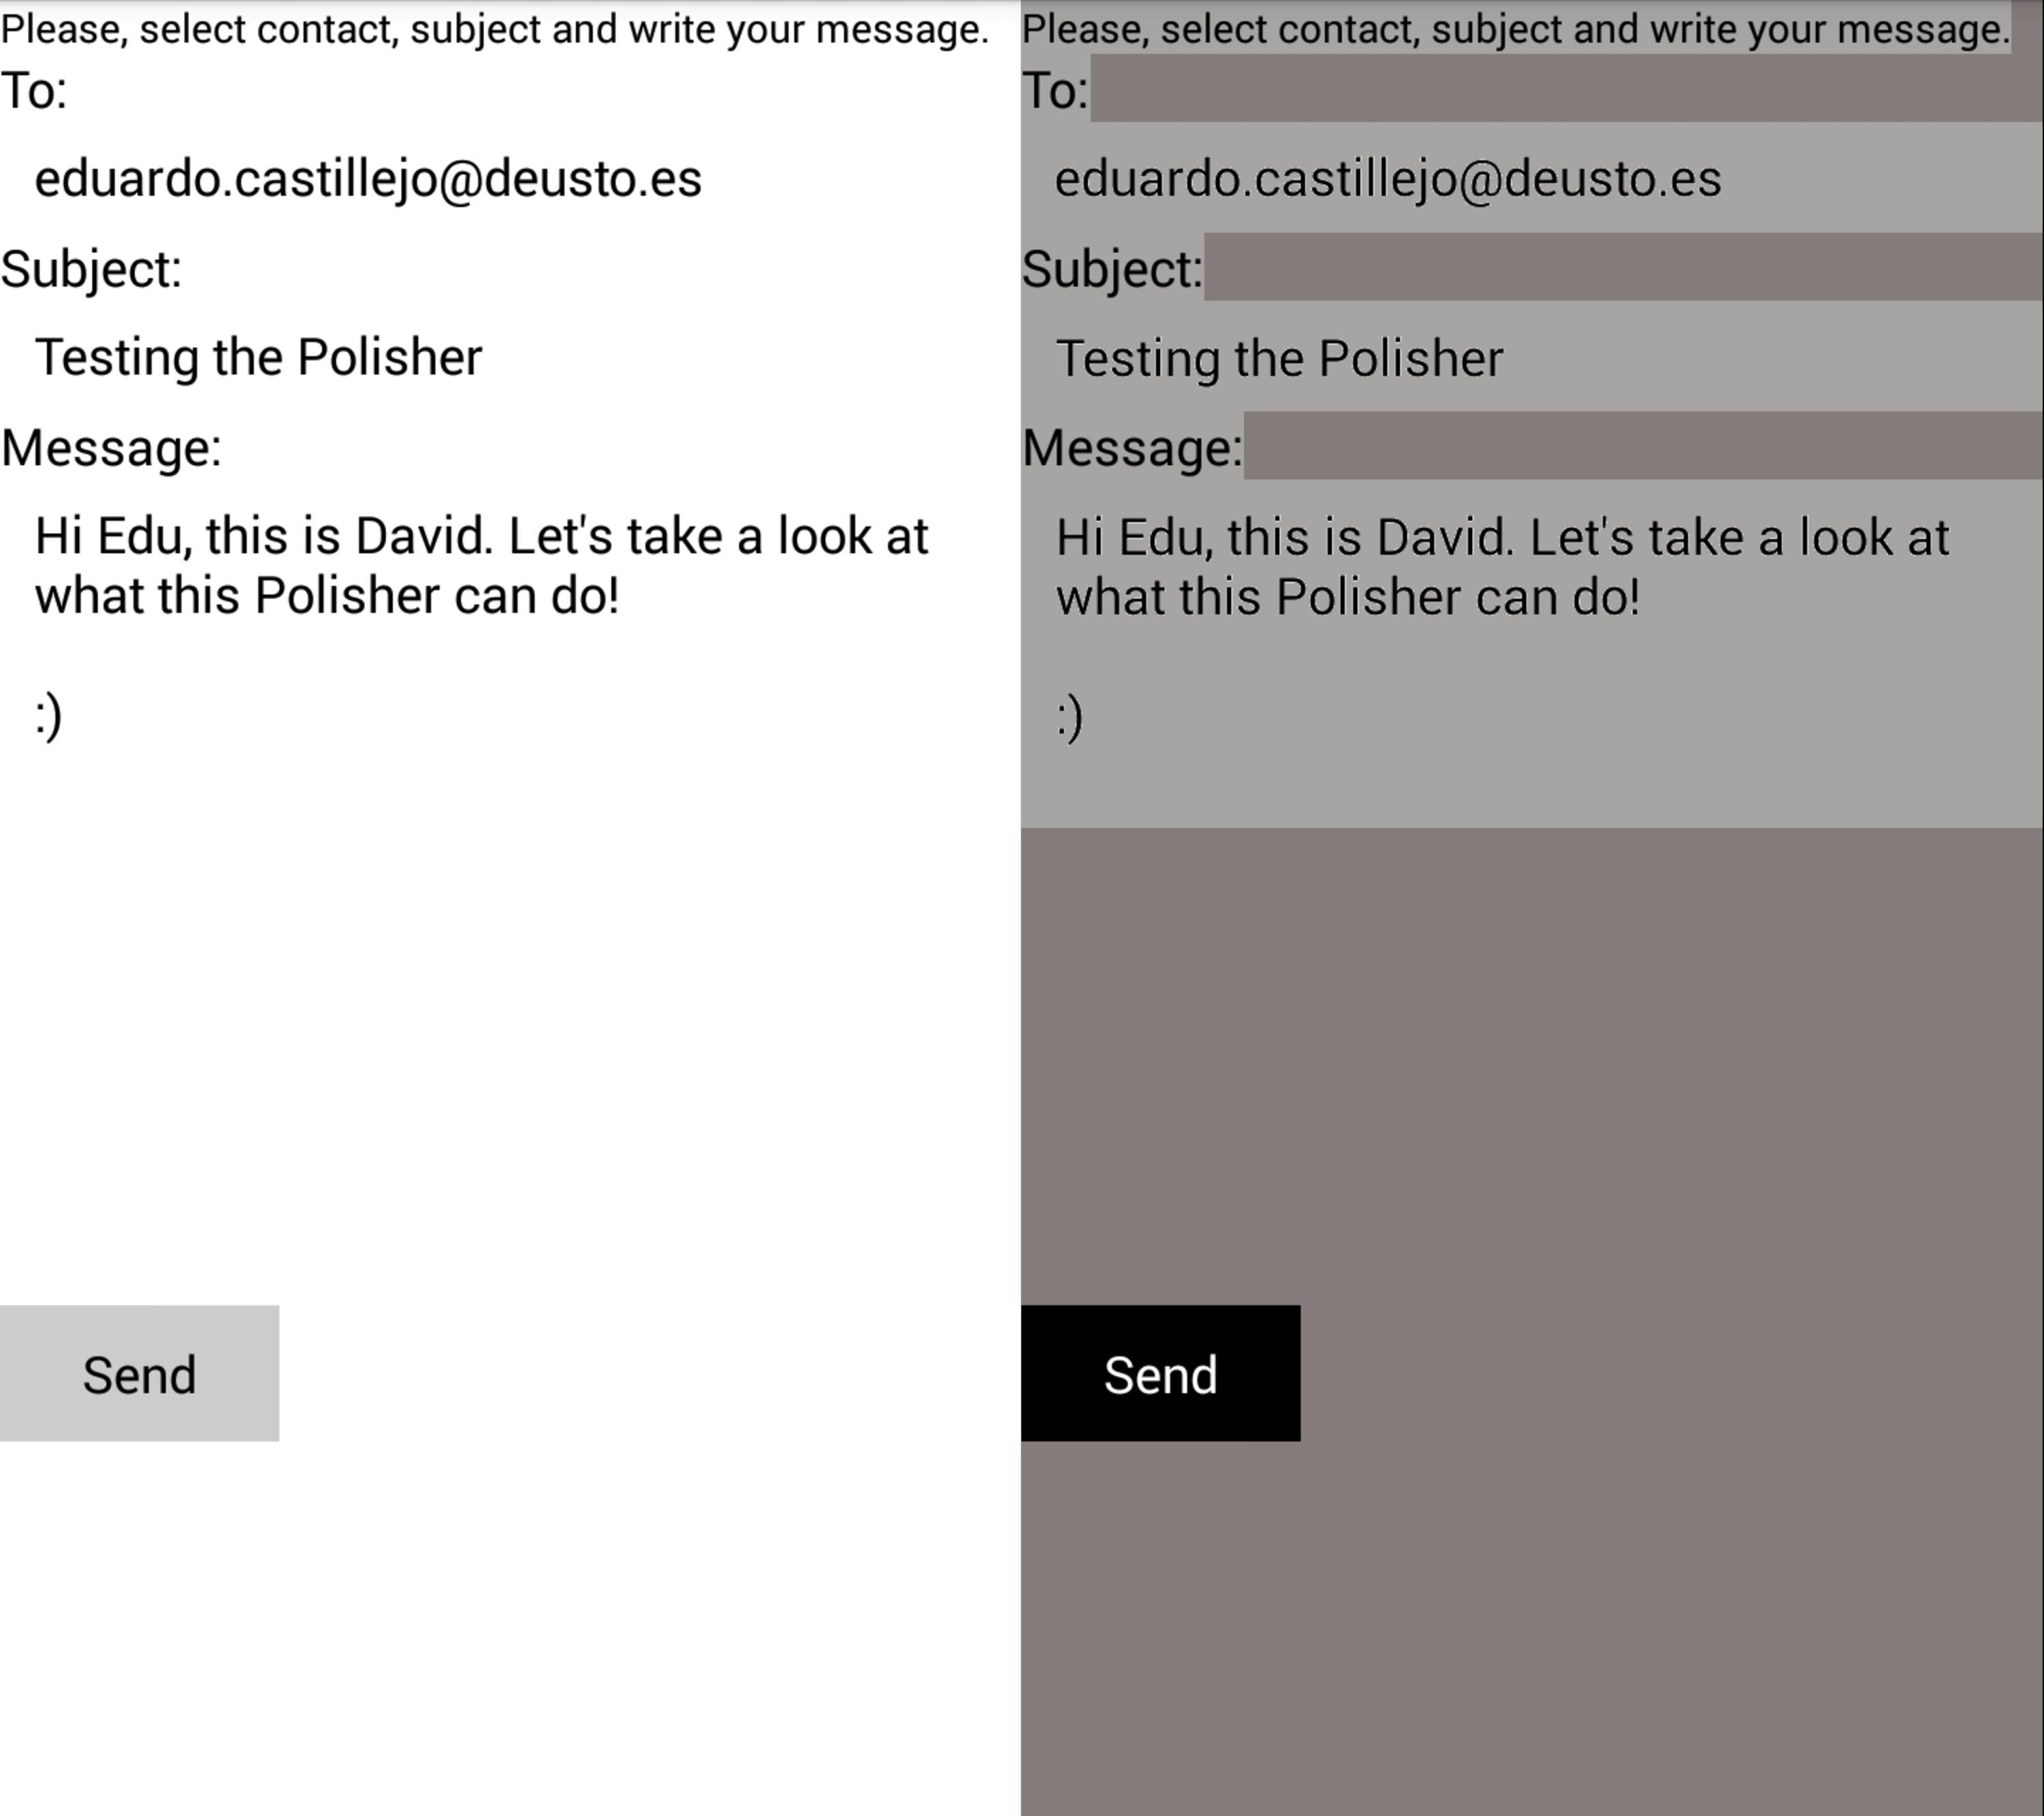
\includegraphics[width=0.65\textwidth]{polisher_scenario.pdf}
\caption{User interface adaptation performed by the Adaptation Engine. On the
left, the default version, without adaptations. On the right, the same 
application adapted by AdaptUI.}
\label{fig:polisher_scenario}
\end{figure}

Thus, David uses his device through the adapted user interface. At this point,
the corresponding interaction model is built by the Adaptation Layer, collecting
the usability metrics shown in Section~\ref{sec:usability_metrics} (see 
Table~\ref{tbl:effectiveness_metrics} and Table~\ref{tbl:productivity_metrics}).
Table~\ref{tbl:model_comparison} shows the used metrics and the computed values
for both the default and the adapted interaction models.

\begin{table}
 \caption{The interaction model computed by the Adaptation Layer. Time ($T$) has
 been measured in seconds.}
 \label{tbl:model_comparison}
 \footnotesize
 \centering
\begin{tabular}{l l l}
  \hline 
  \textbf{Metric} 	& \textbf{Value for the default}& \textbf{Value for the adapted}\\
			& \textbf{interaction model} 	& \textbf{interaction model}	\\
  \hline
  Task effectiveness	& $0.7$				& $0.350$	\\
  ($M1=|1-\Sigma A_{i}|$)\\
  Task completion	& $1$				& $0$		\\
  ($X=A/B$)\\
  Error frequency 	& $0.2$				& $0.562$	\\	%3/15, 18/32 
  ($X=A/T$)\\
  \hline
  Task time		& $15$				& $32$		\\
  ($X=Ta$)\\
  Task efficiency 	& $0.046$			& $0.010$	\\
  ($X=M1/T$)\\
%   Productive proportion\\
%   ($X=Ta/Tb$)\\
  Relative user efficiency & $1.0$			& $0.5$		\\
  ($X=A/B$)\\
  \hline
\end{tabular}
\end{table}

As is shown in Table~\ref{tbl:model_comparison}, the resulting adapted user 
interface provided by AdaptUI does not improve the interaction of the user.
The required time for performing the same task (sending an email) is 32 seconds,
while by default David uses 15 seconds approximately. Thus, the user interface
does not fit the user needs. 

Once the interaction model has been built, the Adaptation Polisher checks the
usability rules set. As detailed in Section~\ref{sec:adaptation_polisher}, these
rules trigger the polisher rules if certain usability ranges are exceeded.
Equation~\ref{ec:usability_rule} shows a usability rule checking the relative
user efficiency of the interaction model.

\footnotesize
\begin{equation} \label{ec:usability_rule}
  \begin{align*} 
  Productivity(?productivity) ∧ hasRelativeEfficiency(?productivity, ?efficiency) ∧\\
  lessThanOrEqual(?efficiency, 0.5) ∧ Polisher(?polisher)\\
  \Rightarrow \\
  launchPolisherRules(?polisher, true)
  \end{align*}
\end{equation}
\normalsize

On the other hand, Equation~\ref{ec:polisher_rule} is triggered by 
Equation~\ref{ec:usability_rule}. In the consequent of this rule there is 
a value of $1.10$. This value means that the size of the views presented in the
previous adapted version of the user interface should be increased in a $10\%$
Hence, the next rule polishes the adapted user
interface.

\footnotesize
\begin{equation} \label{ec:polisher_rule}
  \begin{align*} 
  Polisher(?polisher) ∧ launchPolisherRules(?polisher, true) ∧\\
  errorFrequency(?errorFreq) ∧ greaterThan(?errorFreq, 0.5)\\
  \Rightarrow \\
  setViewSize(1.10)
  \end{align*}
\end{equation}
\normalsize

Thus, the resulting polished user interface is shown in Figure~\ref{fig:polisher_4}.

\begin{figure}
\centering
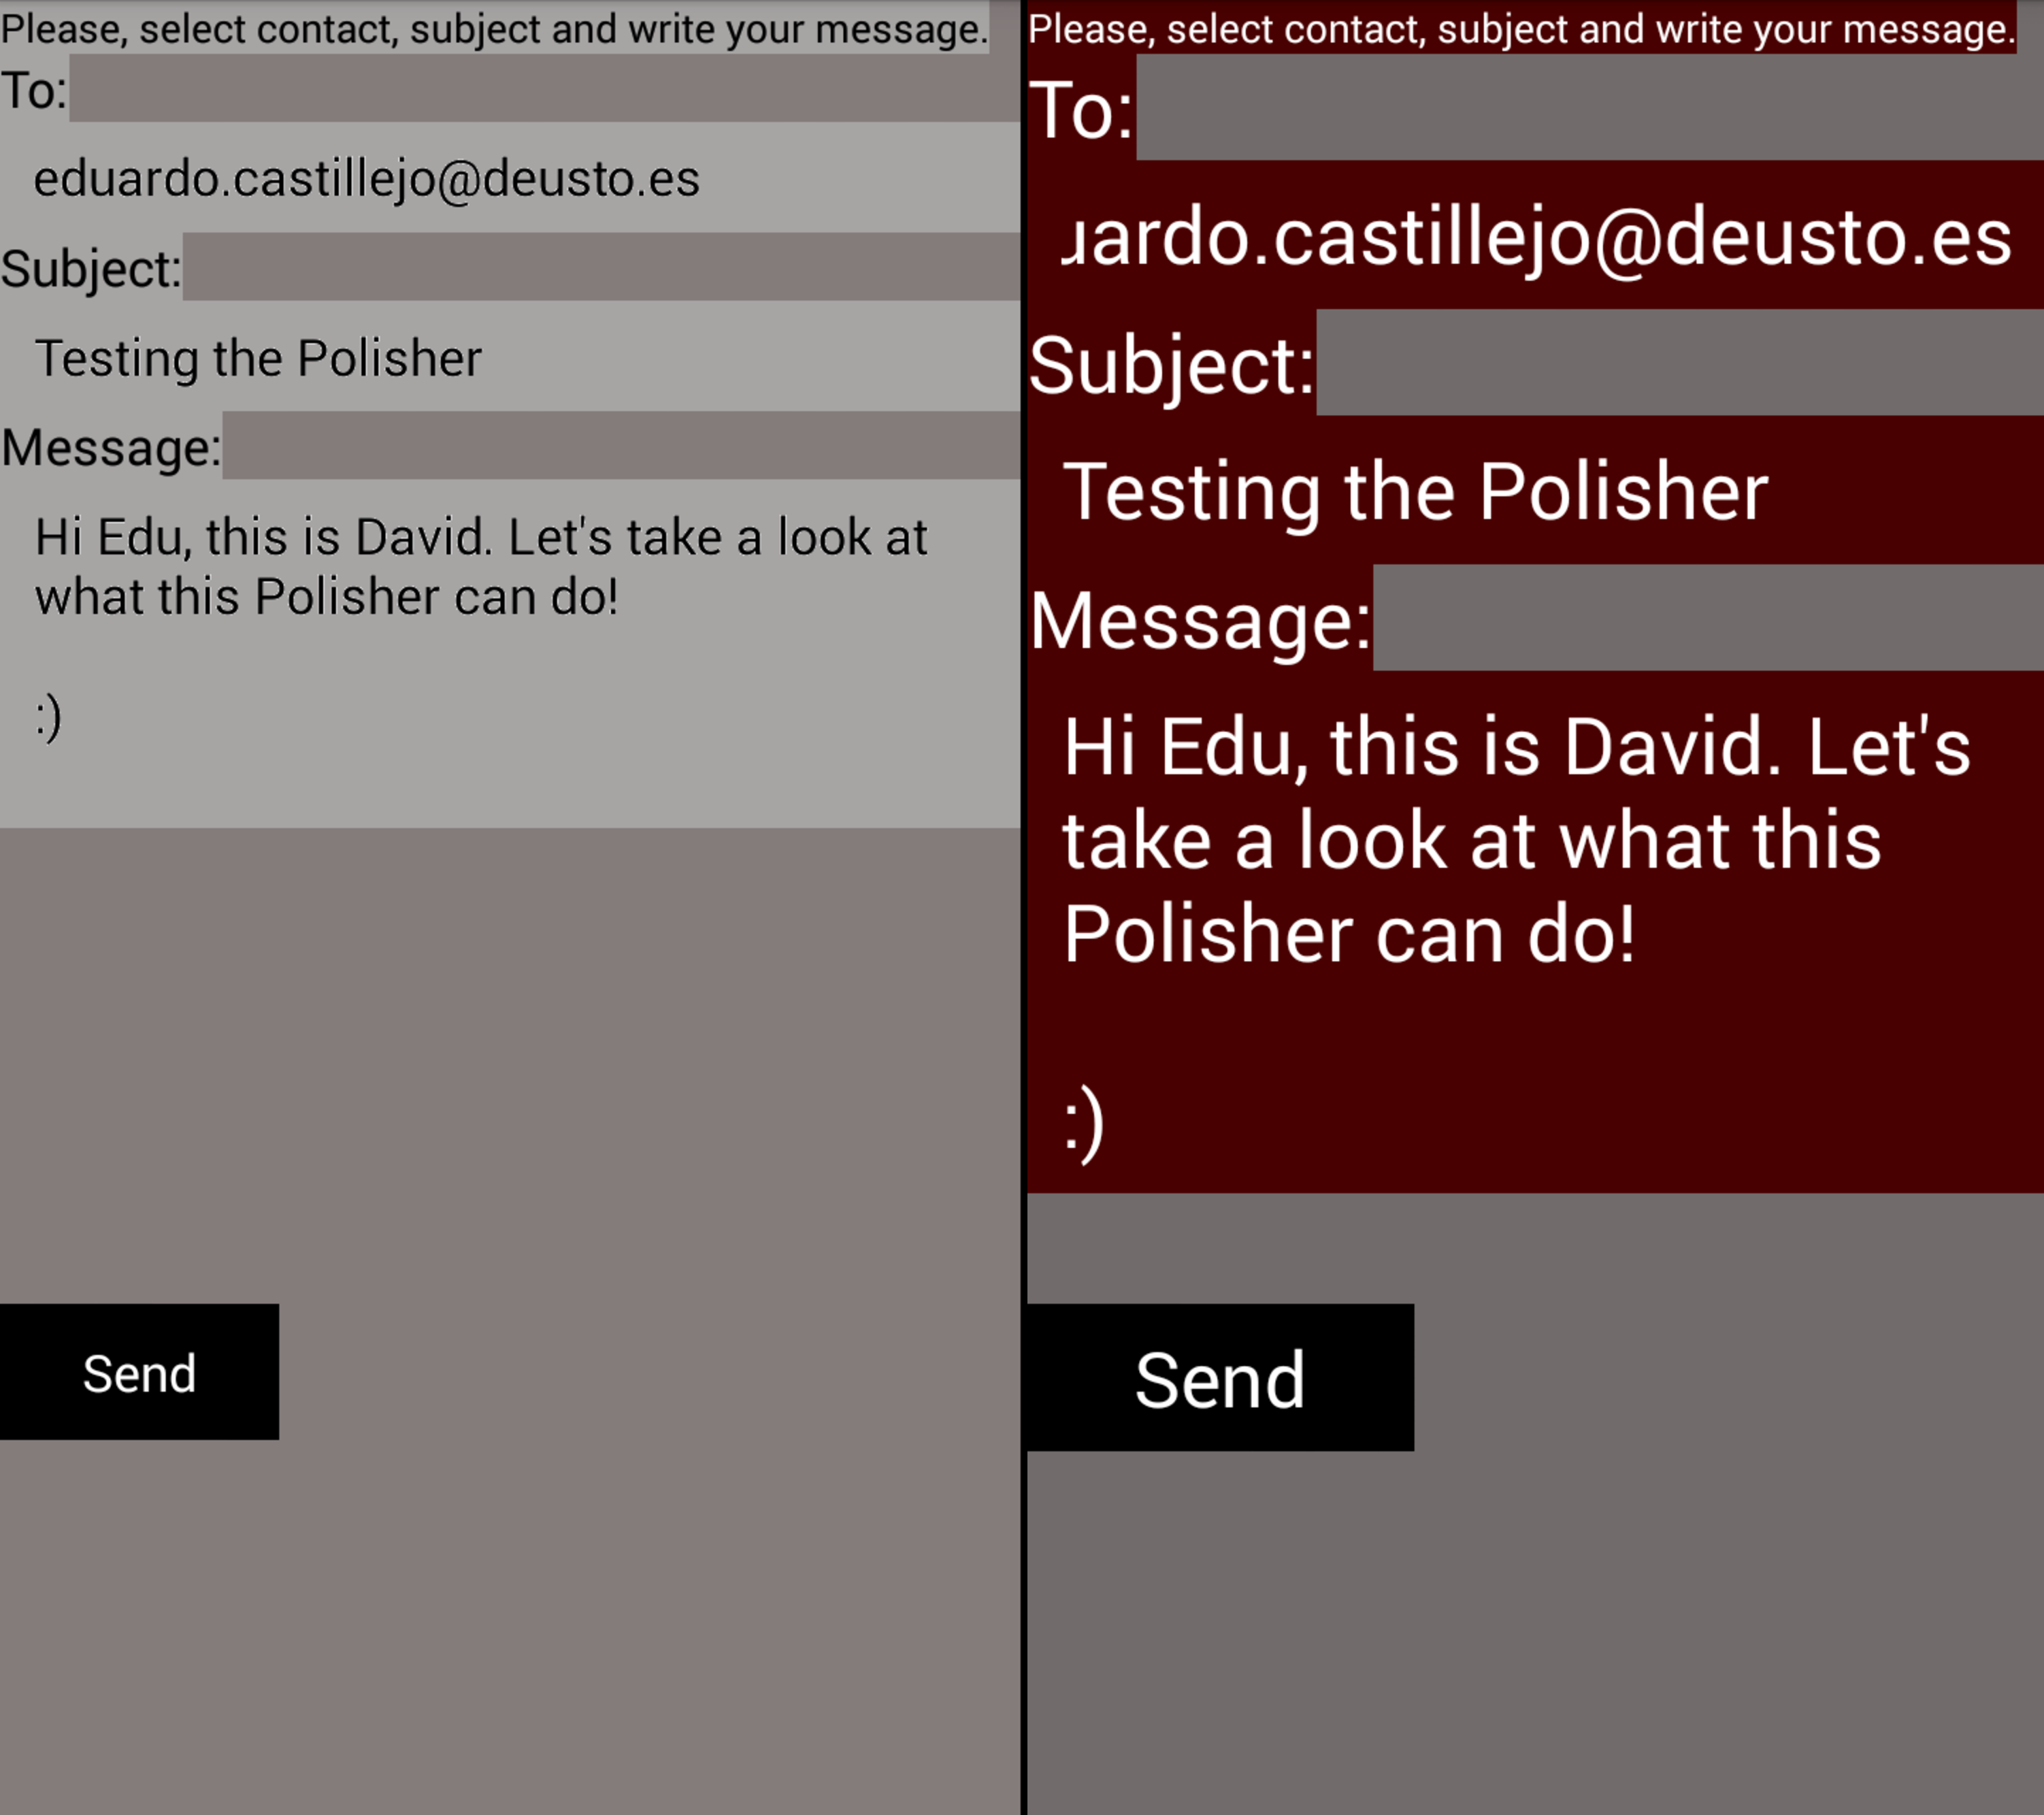
\includegraphics[width=0.65\textwidth]{polisher_4.pdf}
\caption{Polished user interface. On the left, the adapted version. On the 
right, the polished one.}
\label{fig:polisher_4}
\end{figure}

\section{The Application Layer}
\label{sec:application_layer}

The last layer of the AdaptUI architecture is the Application Layer. This layer
aims to ease the use of the AdaptUI platform to developers. To do this, several
tools have been provided. These tools have been designed not only to integrate
AdaptUI within developers' applications (to adapt their user interfaces) but also
to leave in their hands the decision of how to manage the knowledge of the AdaptUI
platform. Thus, through the AdaptUI provided \ac{api}, developers are allowed to:

\begin{enumerate}[label=\alph*)]
 \item Initialize a Pellet reasoner and connect the application to it, loading
 the AdaptUIOnt ontology and its rules.
 
 \item Launch queries about the knowledge stored in the ontology in order to
 adapt the corresponding user interface elements.
 
 \item Generate, change and adapt the knowledge contained in AdaptUI. Classes,
 properties and relationships described in the AdaptUIOnt ontology are fully
 customizable by developers to cover the domain of their adaptation problem.
 
 \item Customize the provided set of rules. The AdaptUI \ac{api} provides a set of
 methods to edit different rules.
\end{enumerate}

The AdaptUI's \ac{api} can be internally divided into two separated \acp{api}. 
The first one, aiming to solve developer's adaptation issues. 
Listing~\ref{lst:api_adaptation} shows an example of an Android activity 
developed using AdaptUI. The second one, with the purpose of adapting the 
knowledge of the domain (see an example in Listing~\ref{lst:api_knowledge}).

\inputminted[linenos=true, fontsize=\footnotesize, frame=lines]{java}{4_system_architecture/api_adaptation.java}
\captionof{listing}{The AbstractActivity class ontology related methods.\label{lst:api_adaptation}}

\inputminted[linenos=true, fontsize=\footnotesize, frame=lines]{java}{4_system_architecture/api_knowledge.java}
\captionof{listing}{Modifying the ontology knowledge with the AdaptUI's \ac{api}.\label{lst:api_knowledge}}


\subsection{Customizing the AdaptUIOnt knowledge}
\label{sec:knowledge_editor}
Ontologies are formal specification of concepts that represent knowledge within
a specific domain. This knowledge is provided through a vocabulary which describes
the types and relationships of the concepts represented in that specific domain.

The knowledge conceptualization is mainly described through classes, attributes,
relations, individuals and axioms: 

\begin{itemize}
  \item Classes represent concepts within the domain. In other words, classes
  describe the type or kind of the members of the class.
  
  \item Each class can have a set of properties or characteristics which describe
  it. These properties are represented through attributes. These attributes
  are also called datatype properties.
  
  \item Relations detail the relationships that the concepts of the ontology
  might share. They are referred as object properties.
  \item Instances are the representation of the concepts of the
  ontology.
  
  \item Finally, axioms, including rules, are assertions that together comprise
  the overall theory that the ontology describes in the current domain.
\end{itemize}

These concepts together build ontologies to represent the knowledge of a domain.
In AdaptUI,the knowledge of a domain is not considered static. Besides, the 
solutions provided in the literature usually do not apply well when changing 
the domain. Therefore, AdaptUI aims to ease the adaptation of the domain 
knowledge through the customization of these concepts. Through a set of methods 
within the AdaptUI \ac{api}, developers are allowed to insert, edit and delete 
classes, attributes, instances and rules. Table~\ref{tbl:api_knowledge} shows 
the available methods for developers to modify the knowledge contained in the 
AdaptUIOnt ontology.

AdaptUI is designed to support several user capabilities, context status and
device characteristics. Nevertheless, regarding the rules set it is impossible
to assume every possible situation and react accordingly. Thus, a set of methods
to create, edit and delete \ac{swrl} rules has been provided. This allows developers
to adapt the AdaptUI platform to new and unexpected situations in the domain
where the platform might not behave properly.

\begin{center}
\footnotesize

\begin{longtable}{l l l l}
  \caption{Knowledge related AdaptUI \ac{api} methods}\\
  \label{tbl:api_knowledge} \\
% \footnotesize
% \centering
%  \begin{tabular}{l l l l}
  \hline 
  \textbf{\ac{api} group} 	& \textbf{Method name} 	& \textbf{Description} 		& \textbf{Input}\\
  \hline
  Classes		& insertClass		& Inserts a new class.		& The namespace and the \\
			& 			& 				& class name.		\\
			& removeClass		& Erases an existing class, its	& The namespace and the \\
			& 			& individuals, attributes and	& class name.		\\
			& 			& relationships with other 	& 			\\
			& 			& classes.			& 			\\
			& editClass		& Changes the name of the class.& The namespace and the \\
			&			& Internally it deletes the 	& new class name.	\\
			&			& class passed as parameter 	&			\\
			&			& and creates a new one.	&			\\
\hline 
  Object 		& insertObjectProperty	& Inserts a new object property	& The namespace and the	\\
  properties		&			& connecting two classes.	&  object property name.\\
			&			&				& It also needs the 	\\
			& 			& 				& namespaces and names of 	\\
			&			&				& the classes that will be 	\\
			& 			& 				& connected. The two set 	\\ 
			&			&				& of classes are passed as 	\\
			& 			& 				& a Map$<$String namespace,	\\
			& 			& 				& String classname$>$.	\\
			& removeObjectProperty	& Erases an existing datatype	& The namespace and the \\
			& 			& property.			& object property name.	\\
			& editObjectProperty	& Changes the name of the 	& The namespace and the \\
			&			& datatype property. Internally & new class name.	\\
			&			& it deletes the property 	& 			\\
			&			& passed as parameter and 	&			\\
			& 			& creates a new one.		& 			\\
  \hline 
  Datatype 		& addDatatypeProperty	& Inserts a new datatype 	& The namespace and the \\
  properties		&			& property assigning a value to & datatype property name.\\
			& 			& a class.			& 			\\
			&			& If it does not exist, it is	& It also needs the namespace 	\\
			&			& created.			& and name of the class \\
			& 			& 				& that will have this property 	\\
			& 			& 				& and the value type.	\\
			& removeDatatypeProperty& Erases an existing datatype	& The namespace and the \\
			& 			& property.			& datatype property name.\\
			& editDatatypeProperty	& Changes the name of the 	& The namespace and the \\
			&			& datatype property. Internally & new class name.	\\
			&			& it deletes the property passed& 			\\
			&			& as parameter and creates 	&			\\
			& 			& a new one.			& 			\\
  \hline 
  Individuals 		& insertIndividual	& Inserts a new individual of a & The name of the 	\\
			&			& concrete class.		& individual and the 	\\
			& 			& 				& namespace and name 	\\
			& 			& 				& of the class.		\\
			& removeIndividual 	& Removes an individual.	& The name of the 	\\
			&			&				& individual to be 	\\
			& 			& 				& deleted.		\\
  \hline 
  Rules 		& insertRule		& Inserts a new rule.		& The name of the 	\\
			&			& 				& rule, the antecedent 	\\
			& 			& 				& and the consequent.	\\
			& removeRule 		& Removes a rule if the rule 	& The name of the rule 	\\
			&			& has a name associated to it.	& to be deleted.	\\
  \hline
% \end{tabular}
\end{longtable}

\end{center}


\section{The Information Flow}
\label{sec:architecture_flow}

Once the AdaptUI's layers and modules have been described, in this section the 
interaction among them and the information flow are reviewed.
Figure~\ref{fig:architecture_flow} shows a diagram with the whole architecture
and data flows.

First, and within the Modelling Layer, the user capabilities and context and
device characteristics are collected by the Capabilities Collector. This module
stores the collected information about these entities in Android using key-value
sets. While the capabilities of the device and several context parameters are
gathered transparently for the user, to collect his/her capabilities the
Capabilities Collector needs the user to complete a profile personalization process.

Once the Capabilities Collector finishes its task, the Semantic Modeller retrieves
the stored information and begins to transform it into semantics using the
AdaptUIOnt ontology. To be able to use semantics and to manipulate the model
and the available knowledge about the entities the Semantic Modeller uses
\textit{Pellet4Android}, which is an Android based port of Pellet.

Next, the Adaptation Engine (within the Adaptation Layer) semantically requests
the last adaptation instructions. These instructions are defined by the rules
triggered when the Semantic Modeller stores the knowledge in the AdaptUIOnt
ontology. Once it is stored, the corresponding rules result into a series of
adaptations. These adaptations, represented through the \textit{Adaptation}
class, are collected by the Adaptation Engine and represented in the user's display.

Once the user receives the corresponding adapted user interface, another Adaptation
Layer's module works in background: the Adaptation Polisher. Actually, this module
starts working from the beginning. Its purpose is to be aware of the user interaction
with the applications. This includes not only the adapted applications but also
the rest of them. Thus, it is able to establish several usability boundaries
under which the user might no be comfortable with. Comparing the user interaction
profile (generated during the usage of default applications under normal
circumstances) and the adapted interaction model (generated during the interaction
with an adapted user interface) this module triggers several instructions to
re-adapt the user interface. These instructions are ruled through the
post-adaptation set of rules.

Finally, within the Application Layer several tools (provided through an \ac{api})
are available for developers to make their applications adaptive and modify the
knowledge which will represent the domain (including concepts, relationships and
rules).

\begin{figure}
\centering
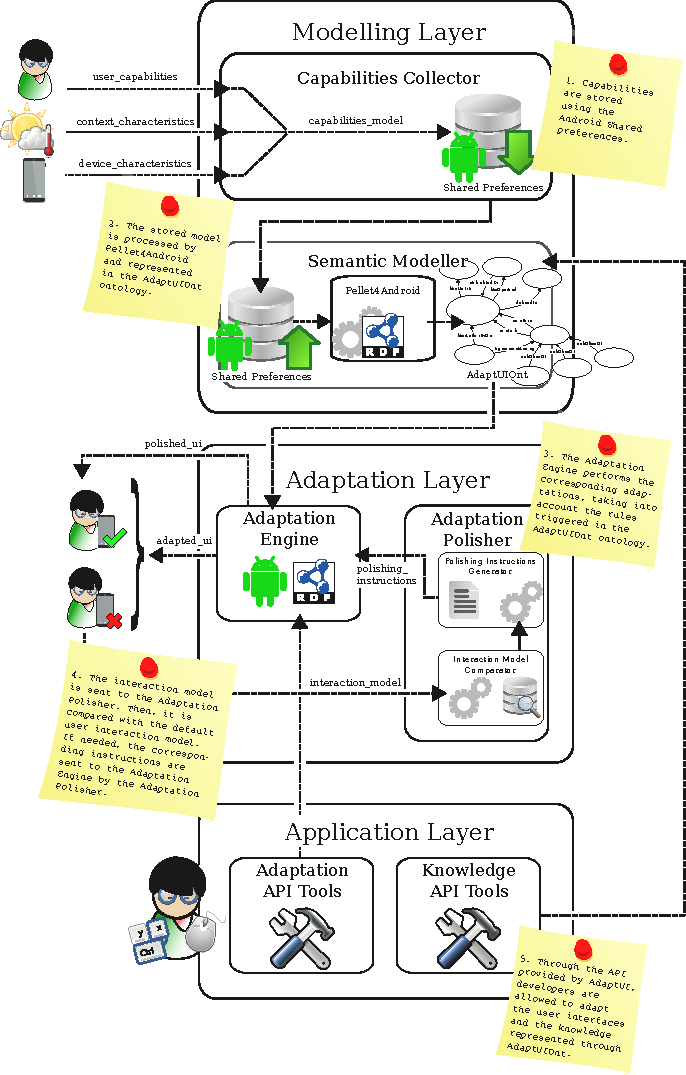
\includegraphics[width=0.85\textwidth]{architecture_flow.pdf}
\caption{The information flow within the AdaptUI platform.}
\label{fig:architecture_flow}
\end{figure}

% \InsertFig{architecture_flow}{fig:architecture_flow}{The information flow within
% the AdaptUI platform.}{}{0.85}{}
% ----------------------------------------------------------------------


\section{A Complete Example}
\label{sec:complete_example}

The modules described in the previous sections of this chapter work together to
provide an adapted user interface for the sensed user's context disabilities. 
In the following lines an example of how this process is carried out is 
presented. The definition of the scenario is shown in Table~\ref{tbl:example_scenario}.
% , and the corresponding non adapted user 
% interface is illustrated by Figure~\ref{fig:example_scenario_default}.

\begin{table}[H]
 \caption{Scenario summary.}
 \label{tbl:example_scenario}
 \footnotesize
 \centering
\begin{tabular}{l l}
  \hline 
				& \textbf{Scenario}		\\
  \hline
  User \\
  \qquad - Personal data 	& Molly, $39$ years old, United States\\
  \qquad - Activity	 	& Phone call			\\
  \qquad - Known disabilities 	& - 				\\
% 				& Hearing loss 			\\
%   \hline
  Context \\
  \qquad - Location 		& Relative: Plentzia, Spain  	\\
				& 				\\
  \qquad - Time			& $14$:$35$ 			\\
  \qquad - Brightness		& $30,000$ \ac{lx}		\\
  \qquad - Noise		& $80$ \acp{db}			\\
  \qquad - Temperature		& $28$ ºC 			\\
%   \hline
  Device 			& Samsung Galaxy SII 	 	\\
				& Battery: $55$\%			\\
  \hline
\end{tabular}
\end{table}

The following lines detail the adaptation process, highlighting each layer's and
module's goal and behaviour. As the user is trying to perform a phone call, the 
corresponding default user interface is shown in Figure~\ref{fig:example_scenario_default}.

\begin{figure}[H]
\centering
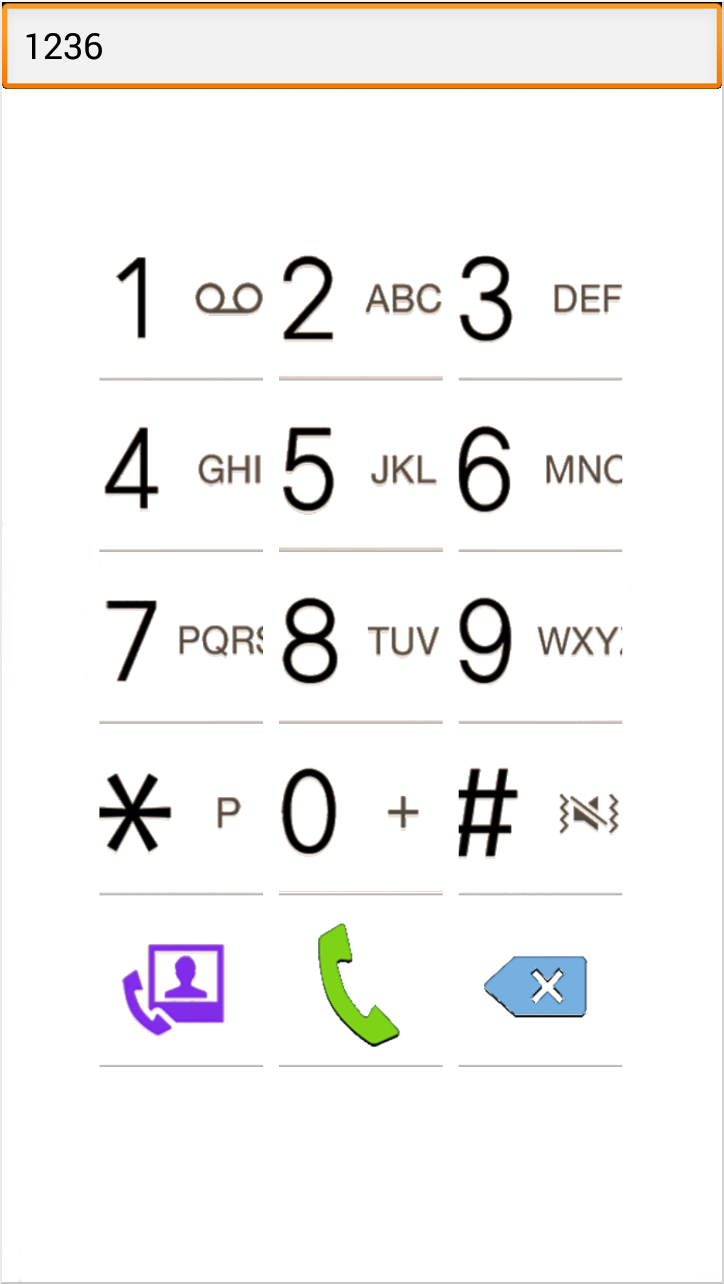
\includegraphics[width=0.35\textwidth]{example_scenario_default.png}
\caption{A simple phone call application user interface.}
\label{fig:example_scenario_default}
\end{figure}

\begin{itemize}
%%%%%%%%%%%%%%%%%%%%%%%%%%%%%%%%%%%%%%%%%%%%%%%%%%%%%%%%%%%%%%%%%%%%%%%%%%%%%%%%
%%%%%%%%%%%%%%%%%%%%%%%%%%Modelling Layer%%%%%%%%%%%%%%%%%%%%%%%%%%%%%%%%%%%%%%%
%%%%%%%%%%%%%%%%%%%%%%%%%%%%%%%%%%%%%%%%%%%%%%%%%%%%%%%%%%%%%%%%%%%%%%%%%%%%%%%%
  \item The Modelling Layer aims to build a semantic model of the user, context
  and device, based on the interaction characteristics available in the current
  situation. For further details of the Modelling Layer see Section~\ref{sec:modelling_layer}.
  
  \begin{itemize}
    %Capabilities Collector%%%%%%%%%%%%%%%%%%%%%%%%%%%%%%%%%%%%%%%%%%%%%%%%%%%%%
    \item First, the user has to use the Capabilities Collector. As explained in 
    Section~\ref{sec:capabilities_collector}, this software module collects non 
    physiological capabilities of the user, gathers different variables of the 
    current context, and identifies several device characteristics. An example of 
    the Capabilities Collector is given through 
    Figure~\ref{fig:capabilities_collector_scenario}. Through a series of
    activities, the user is requested to dynamically configure different user 
    interface components taking into account the current scenario characteristics. 
    Each activity presents different user interface views, and the user's
    interaction decisions are stored in an Android SharedPreferences model.
    This model is easy to maintain and manipulate, and it serves as input for
    the next module. The user, context and device profiles are detailed in 
    Table~\ref{tbl:profiles}.
    
\begin{figure}
\centering
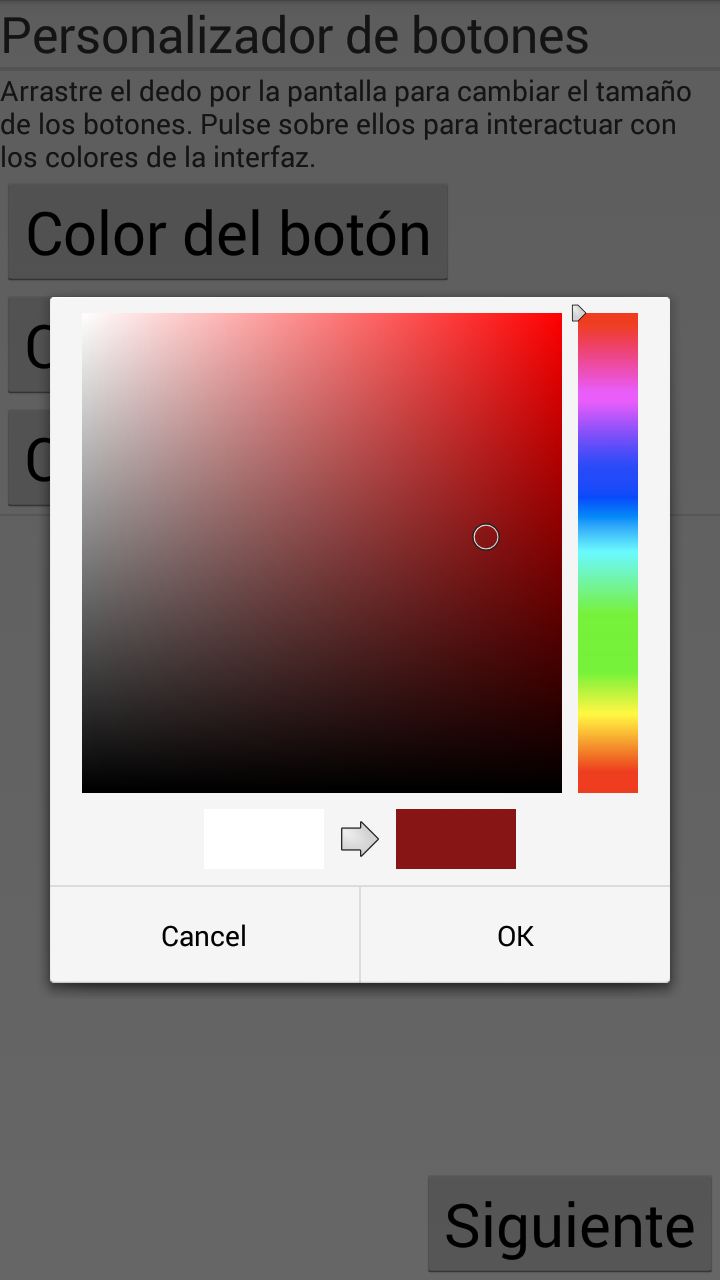
\includegraphics[width=0.35\textwidth]{capabilities_collector_scenario.png}
\caption{A user configuring the buttons colour set through the Capabilities Collector.}
\label{fig:capabilities_collector_scenario}
\end{figure}
    
\begin{table}
 \caption{User, context and device profiles after using the Capabilities Collector.
 The class (*) is translated to a semantic representation in the AdaptUIOnt ontology.
 It is not represented in the SharedPreferences model. The colour set (*) represents
 the whole colour configuration that the user specifies for the corresponding
 views, including the background colours, text colours and so on.}
 \label{tbl:profiles}
 \footnotesize
 \centering
\begin{tabular}{l l l l}
  \hline 
  \textbf{Entity}& \textbf{Class(*)}& \textbf{SharedPreferences} & \textbf{Value}\\
		& 		& \textbf{property} 		& \\
  \hline
  User 		& Interface 	& \textit{input}		& default	\\
		& 		& \textit{output} 		& default	\\
		& View		& \textit{colourSet(*)}		& default	\\
		& Display 	& \textit{minBrightness}	& $9$		\\ 
		& 		& \textit{maxBrightness}	& max		\\
		& Audio 	& \textit{minVolume}		& $4$		\\
		& 		& \textit{maxVolume} 		& max		\\
		& Other 	& \textit{language}		& English	\\
		& 		& \textit{vibration} 		& true 		\\
		
  Context	& Brightness	& \textit{brightness}		& $30,000$	\\
		& Noise		& \textit{noise}		& $80$		\\
		& Time		& \textit{time}			& $14$:$35$	\\
		& Location	& \textit{city}			& Plentzia	\\
		&		& \textit{country}		& Spain		\\
		&		& \textit{longitude}		& $43.414353$	\\
		&		& \textit{latitude} 		& $-2.944183$	\\
  Device	& \ac{os}	& \textit{osVersion}		& $4.1.2$	\\
		& Battery	& \textit{battery}		& $55$		\\
		& Volume	& \textit{maxVolume}		& $12$		\\
		& Brightness	& \textit{maxBrightness}	& $15$		\\
		& DeviceScreenResolution & \textit{resolution}	& $480×800$	\\	
  \hline
\end{tabular}
\end{table}

    %Semantic Modeller%%%%%%%%%%%%%%%%%%%%%%%%%%%%%%%%%%%%%%%%%%%%%%%%%%%%%%%%%%
    \item Once the interaction with the Capabilities Collector is finished, the
    Semantic Modeller (see Section~\ref{sec:semantic_modeller}) uses the 
    SharedPreferences stored model and stores it as a semantic representation of 
    this model in the AdaptUIOnt ontology. This is performed thanks to the 
    \textit{Pellet4Android} mobile semantic engine, which allows to manipulate 
    semantic knowledge in Android. Storing in the ontology requires more time 
    than using SharedPreferences. Thus, the last operation in the Modelling Layer 
    is the semantic storage. The most significant represented characteristics 
    are shown in Table~\ref{tbl:capabilities_collector_scenario}. Those 
    characteristics that are not present in Table~\ref{tbl:profiles} are computed 
    by the pre-adaptation. For example, Equation~\ref{ec:pre_rule_1} updates the 
    \textit{userAuxDisplayHasApplicable} datatype property by checking if the 
    user interacts with the Capabilities Collector in a \textit{default} manner.
    
    \footnotesize
    \begin{equation} \label{ec:pre_rule_1} 
    \begin{align*} 
    adaptui:UserAux (?uaux) ∧ adaptui:UserCharacteristics (?user) ∧ \\
    adaptui:Interface (?interf) ∧ adaptui:Input (?input) ∧ \\
    userHasInterface (?user, ?interf) ∧ interfaceHasInput (?interf, ?input) ∧\\
    swrlb:equal ("default") \\    
    \Rightarrow \\
    adaptui:userAuxDisplayHasApplicable (?uaux, true)
    \end{align*}
    \end{equation}
    \normalsize
    
    

  \end{itemize}

\begin{table}
 \caption{User, context and device profiles as represented in the AdaptUIOnt ontology.}
 \label{tbl:capabilities_collector_scenario}
 \footnotesize
 \centering
\begin{tabular}{l l l l}
  \hline 
  \textbf{Entity}& \textbf{Class} & \textbf{Property} 			& \textbf{Value}\\
  \hline
  User 		& Display 	& \textit{userDisplayIsApplicable} 	& true		\\% Esto se saca con reglas
		& 		& \textit{userDisplayBrightnessIsStatic}& false		\\
		& Audio 	& \textit{userDisplayApplicableIsStatic}& false		\\
		& 		& \textit{userAudioHasApplicable} 	& true		\\
		& 		& \textit{userAudioApplicableIsStatic} 	& false		\\
		& 		& \textit{userAudioHasVolume}  		& $4$ 		\\
		& Interface 	& \textit{userInterfaceInput}		& default	\\
		& 		& \textit{userInterfaceOutput} 		& default	\\
% 		& Experience	& \textit{userHasExperience} 		& high		\\
		& View		& \textit{userViewIsStatic}		& false		\\
		& Other 	& \textit{userHasLanguage}		& English	\\
		& 		& \textit{vibration} 			& true 		\\
  Context	& Brightness	& \textit{contextHasBrightness}		& $30,000$	\\
		& Noise		& \textit{contextHasNoise}		& $80$		\\
		& Time		& \textit{contextHasTime}		& $14$:$35$	\\
		& Location	& \textit{contextHasRelativeLocationCity}& Plentzia	\\
		&		& \textit{contextHasRelativeLocationCountry}& Spain	\\
		&		& \textit{contextHasAbsoluteLocationLongitude}& $43.414353$\\
		&		& \textit{contextHasAbsoluteLocationLatitude} & $-2.944183$\\
  Device	& Software (\ac{os})& \textit{deviceHasOSVersion}	& $4.1.2$	\\
		& Hardware (Battery)& \textit{deviceHasBattery}		& $55$		\\
		& (Volume)	& \textit{deviceHasMaxVolume}		& $12$		\\
		& (DeviceScreenResolution) & \textit{deviceHasResolution}& $480×800$	\\	
  \hline
\end{tabular}
\end{table}

%%%%%%%%%%%%%%%%%%%%%%%%%%%%%%%%%%%%%%%%%%%%%%%%%%%%%%%%%%%%%%%%%%%%%%%%%%%%%%%%
%%%%%%%%%%%%%%%%%%%%%%%%%%Adaptation Layer%%%%%%%%%%%%%%%%%%%%%%%%%%%%%%%%%%%%%%
%%%%%%%%%%%%%%%%%%%%%%%%%%%%%%%%%%%%%%%%%%%%%%%%%%%%%%%%%%%%%%%%%%%%%%%%%%%%%%%%
  \item After storing the semantic model in the AdaptUIOnt ontology, it is sent
  to the the Adaptation Layer. This layer aims to lead the dynamic adaptation of
  the elements presented in the user interface.
  
  \begin{itemize}
    %Adaptation Engine%%%%%%%%%%%%%%%%%%%%%%%%%%%%%%%%%%%%%%%%%%%%%%%%%%%%%%%%%%
    \item The Adaptation Engine loads, as input, the stored AdaptUIOnt model, 
    and it executes the corresponding adaptation rules defined by the developer. 
    Once the rules have been executed, the resulting user interface is dynamically 
    updated and presented to the user. Equation~\ref{ec:adap_rule_8} shows how
    the views are updated due to the context brightness. The resulting adapted
    user interface is shown in Figure~\ref{fig:example_scenario_default_vs_adapted}.

    \footnotesize
    \begin{equation} \label{ec:adap_rule_8} 
    \begin{align*} 
    adaptui:Button (?b) ∧ adaptui:ContextCharacteristics(?c) ∧ umo:Light (?light) ∧ \\  
    umo:PhysicalEnvironment (?pe) ∧ contextHasPhysicalEnvironment (?c, ?pe) ∧ \\ 
    lightHasBrightness (?light, ?value) ∧ physicalEnvironmentHasLight (?pe, ?light) ∧ \\
    swrlb:greaterThanOrEqual (?value, 20000) \\
    \Rightarrow \\
    adaptui:buttonHasBackgroundColor (?b, -16711936)
    \end{align*}
    \end{equation}
    \normalsize
    
    \begin{figure}
    \centering
    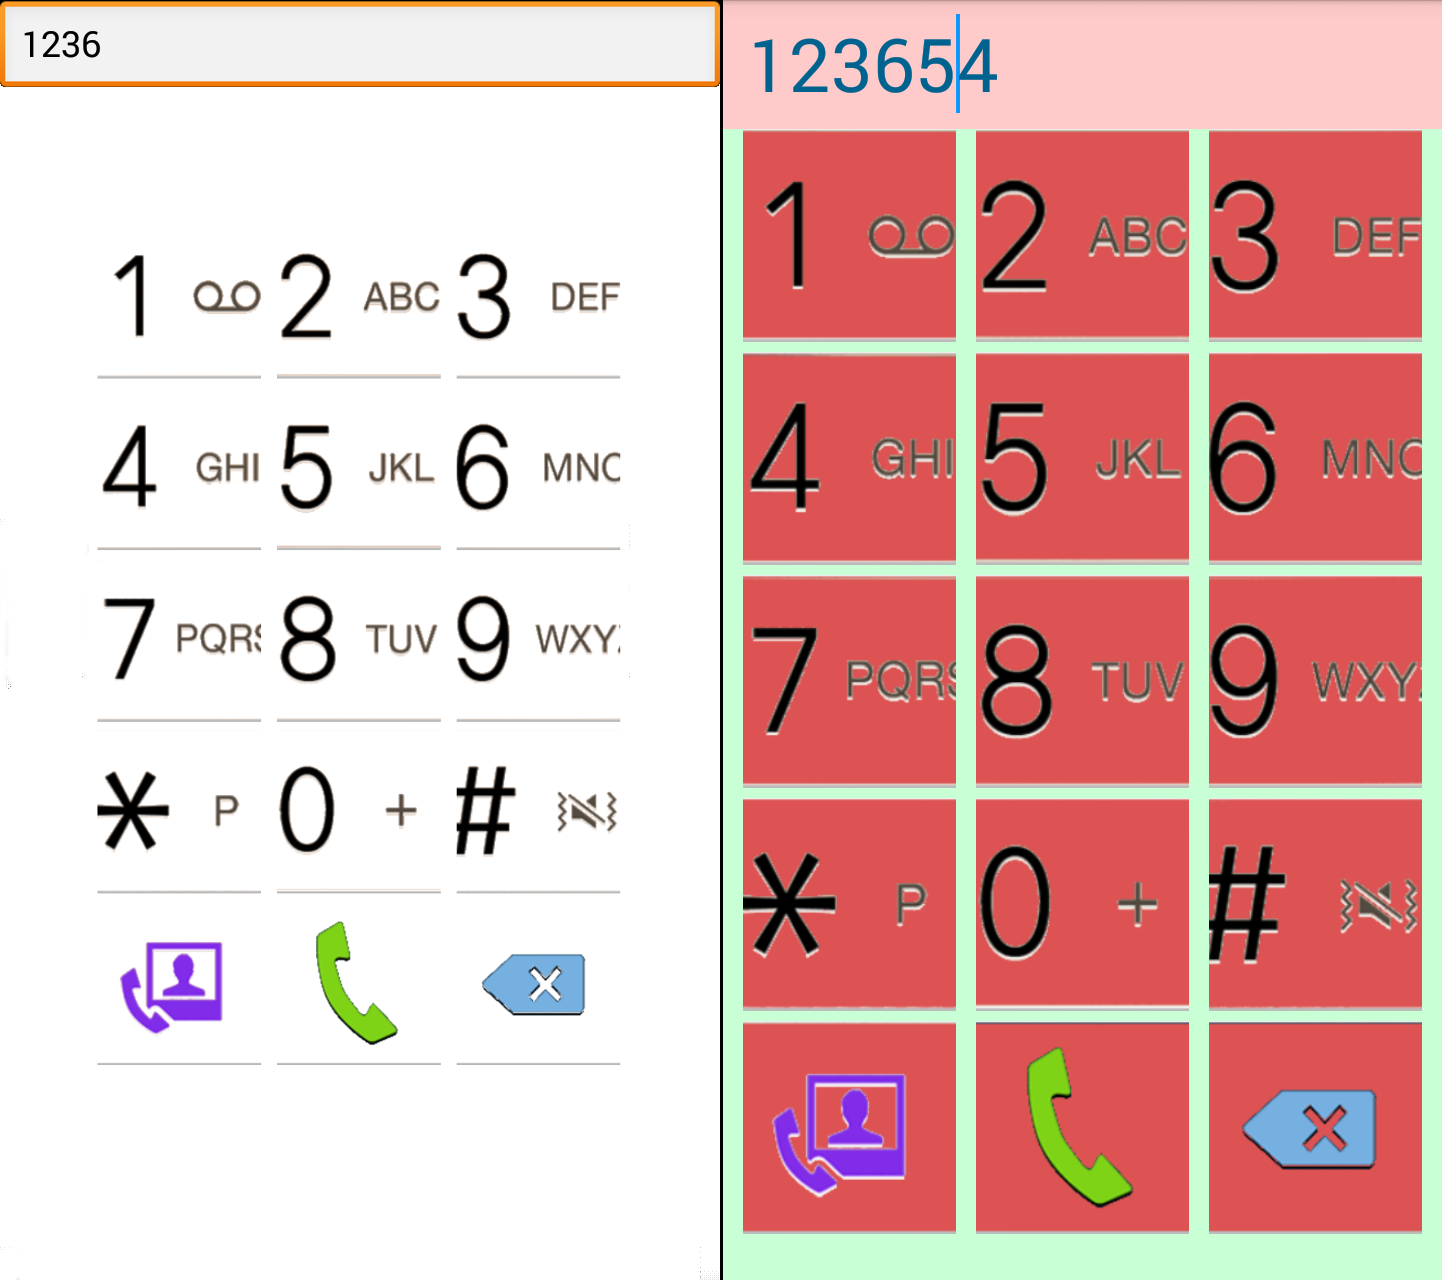
\includegraphics[width=0.50\textwidth]{example_scenario_default_vs_adapted.png}
    \caption{The default user interface (left) and the adapted user interface (right).}
    \label{fig:example_scenario_default_vs_adapted}
    \end{figure}
    
    %Adaptation Polisher%%%%%%%%%%%%%%%%%%%%%%%%%%%%%%%%%%%%%%%%%%%%%%%%%%%%%%%%
    \item Finally, the Adaptation Polisher monitors the usability of the adapted
    user interface. To safeguard this usability it builds and compares two
    interaction models. The first one is built with the usability metrics detailed
    in Section~\ref{sec:usability_metrics} under default circumstances. This means
    that this model is fully accessible by the user in many contexts. The second 
    model, is built from the same usability metrics but taking into account the 
    adapted user interface. The Interaction Model Comparator executes the following
    interaction rules, which aim to evaluate the usability metrics differences
    between the two interaction models. Once these rules are executed, their
    results update the last adaptation of the user interface if needed. The
    polished user interface is compared with the adapted one in 
    Figure~\ref{fig:example_scenario_adapted_vs_polished}. In the presented
    scenario, the Equation~\ref{ec:pre_rule_8} updates polishes the button's
    text as follows: 

    \footnotesize
    \begin{equation} \label{ec:pre_rule_8} 
    \begin{align*} 
    adaptui:Button (?b) ∧ adaptui:Usability (?u) ∧ adaptui:EfficiencyMetric (?em) ∧ \\
    usabilityHasEfficiencyMetric (?u, ?em) ∧ swrlb:greaterThanOrEqual (?value, 0.5) ∧ \\
    efficiencyMetricHasTaskEffectiveness (?em, ?value)\\
    \Rightarrow \\
    adaptui:buttonHasTextColor (?b, 16777215)
    \end{align*}
    \end{equation}
    \normalsize

    \begin{figure}
    \centering
    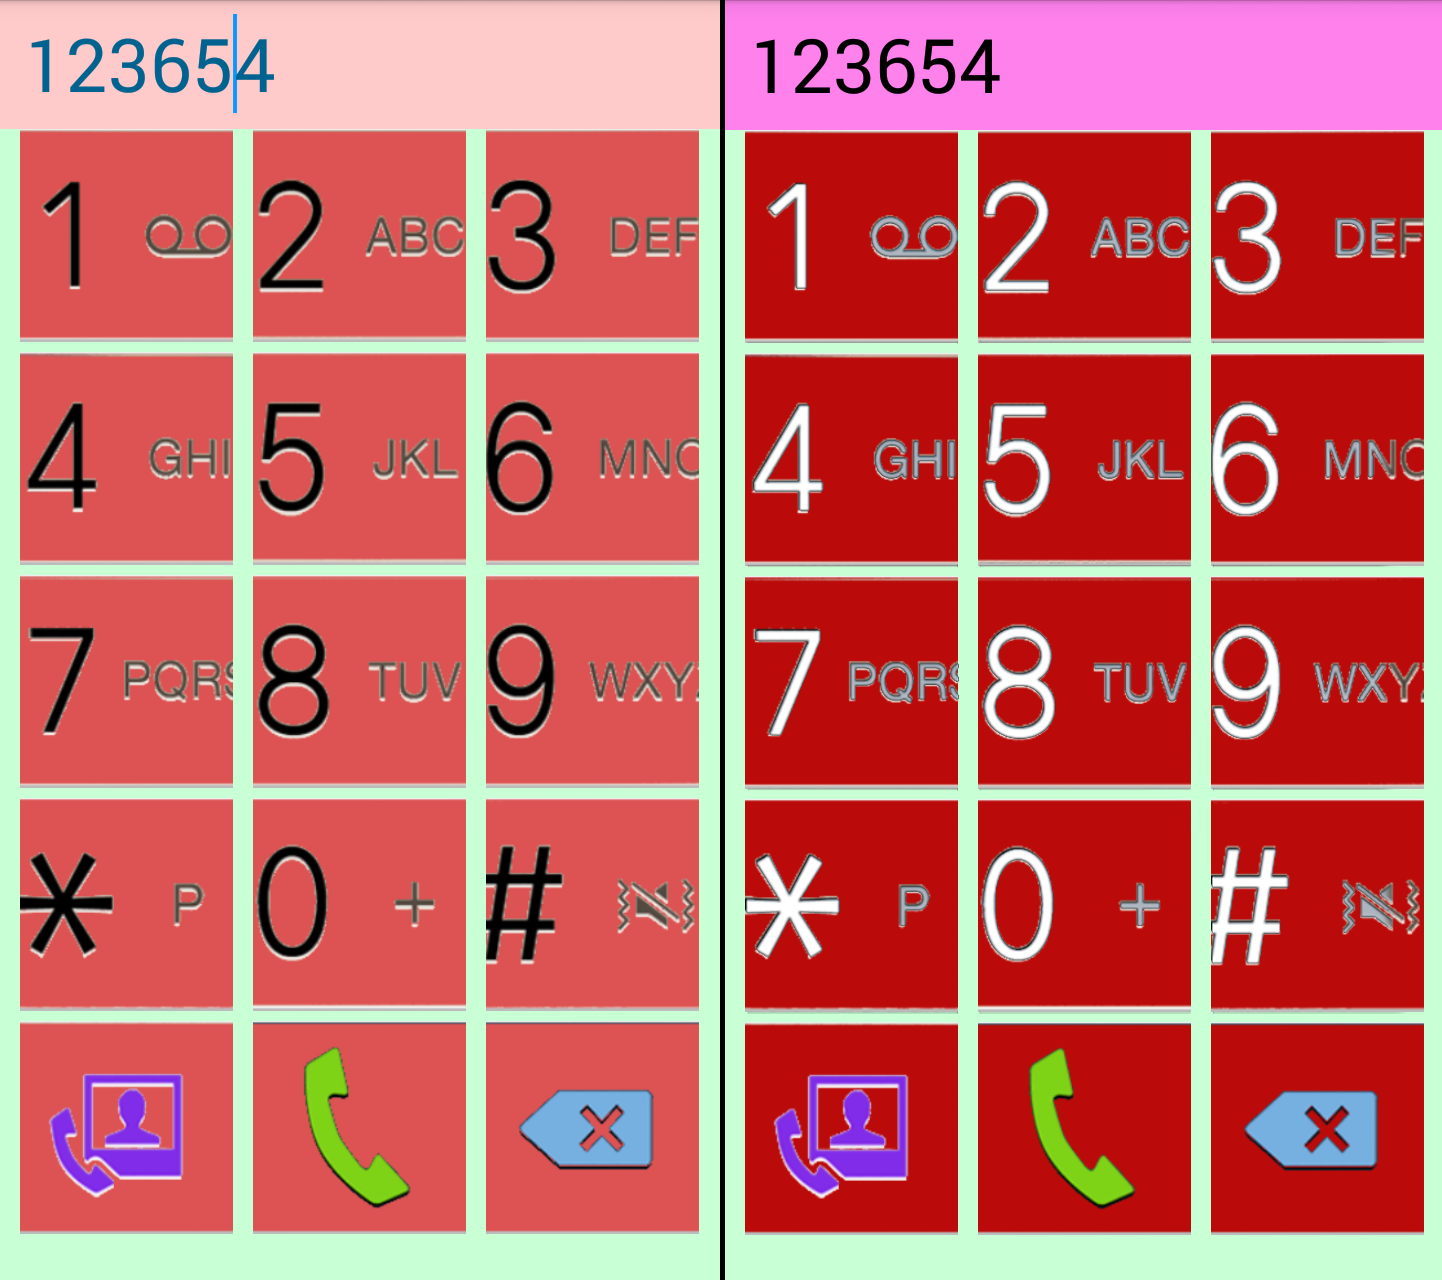
\includegraphics[width=0.50\textwidth]{example_scenario_adapted_vs_polished.png}
    \caption{The adapted user interface (left) and the polished user interface (right).}
    \label{fig:example_scenario_adapted_vs_polished}
    \end{figure}

  \end{itemize}

\end{itemize}

As this example demonstrates, the polisher rules allow the developer to keep
improving the adapted user interfaces. This is carried out by maintaining both
default and adapted interaction models which are based on the usability metrics
detailed in Section~\ref{sec:usability_metrics}.

% Modelling Layer
% - Capabilities Collector
% 1. Llegan las capacidades.
% 2. Se genera el modelo.
% 3. Se guarda en formato SharedPreferences.
% - Semantic Layer
% 4. Se guarda en formato semántico.
% 
% Adaptation Layer
% - Adaptation Engine
% 1. Se analiza el modelo semántico.
% 2. Se ejecutan las reglas correspondientes.
% 3. Se actualiza la interfaz con la nueva adaptación resultante.
% - Adaptation Polisher
% 1. Se genera el modelo de interacción.
% 2. Se ejecutan las reglas de interacción.
% 3. Se envían los resultados al Polishing instructions Generator.
% 4. Se ejecutan las reglas de polishing.
% 5. Se envía al Adaptation Engine la interfaz a adaptar.
